\documentclass[openany]{book}
\usepackage{ln}

\title{UC Berkeley Self-Study/Review Notes: Machine Learning}
\author{Dun-Ming Huang}
\pgfplotsset{compat=1.18}
\setcounter{chapter}{0}

\begin{document}
\maketitle
\setcounter{tocdepth}{1}
\tableofcontents
%\begin{comment}
\part{Training a Model: A Taste of the Fundamentals}
\chapter{DATA C100: Introduction to Modeling}

\section{Motivation}
A \textbf{model} is an idealized representation of a system, which are mostly mathematical. Their mathematical properties lend us the computational opportunity to abstract a system in a computational space! \\
And in general, the machine learning works we perform in DATA C100 lend strength from constructions of models that allow us to predict new values from old data. \\
Outside the context of machine learning, there are a few categories of models that human history has used:
\begin{bindenum}
    \item \textbf{Deterministic Physical (Mechanical) Models}, such as kinematics equations.
    \item \textbf{Probabilistic Models}, which models how random processes can evolve.
    \item \textbf{Statistical Models}, which associates variables via statistical analysis.
    \item \textbf{Informal Models}, which are essentially stories or human-understandable descriptions of a complex phenomenon. Many pictographics might be an informal model.
\end{bindenum}
The introduction towards several categories of models only reinforce the idea that it is used for understanding the world as a complex phenomenon as well as providing predictions towards unseen cases. \\
Quite frequently, we would like to create models that are simple and interpretable, when we attempt to understand the association between different variables.
But when we attempt to make extremely accurate preditcions, we would also risk providing an uninterpretable model whose complexity supports its performance. \\
Both directions of modeling in terms of interpretability have been used, and made their successes in each of their mission. Notably, complex models occur a lot in deep learning. \\

\section{A Demonstration: Simple Linear Regression}

\subsection{What is a Regression Line?}
Suppose we have a crowd of data points spread across a 2D plot, which we call a scatterplot, and we want to predict one dimension of the data point from another, then we may use a regression line:
\begin{ln-define}[sidebyside]{Regression Line}{}
    \begin{center}
        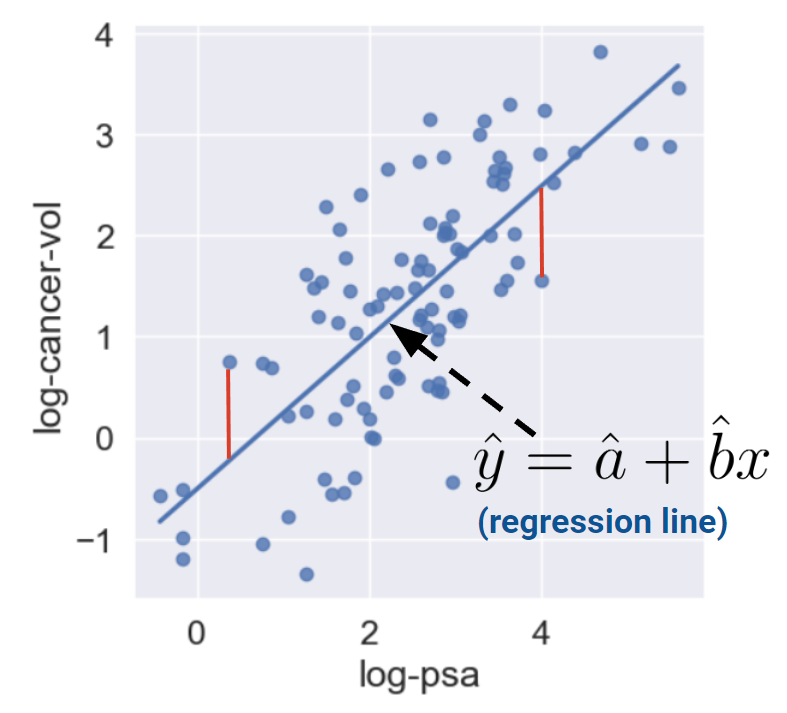
\includegraphics[scale=0.4]{figs/ln01/regression-line.png}
    \end{center}
    \tcblower
    A \textbf{Regression Line} is a linear model that attempts to predict a feature of a specific data-point via a linear combination of other features.
\end{ln-define}
For now, let us simplify our description: ``We would like to predict $y$ by $x$''. \\
The way we predict is by assuming there is a coefficient $a$ and $b$ such that:
\[y = a + bx\]
would accurately predict $y$ for any provided $x$. \\
The most accurate parameter of this line would be denoted as $\hat{a}$ and $\hat{b}$, and the prediction following these best parameters would be denoted as $\hat{y}$, hence the regression line equation:
\[\hat{y} = \hat{a} + \hat{b}x\]

Each dataset that we attempt to apply a regression line onto has a specific statistic called \textbf{correlation}:
\begin{ln-define}{Pearson's Correlation Coeffcient}{}
    A \textbf{correlation} (denoted as $r$), formally known as the ``Pearson's Correlation Coeffcient'', quantifies how linearly associated two variables $x$ and $y$ may be via the following formula:
    \[r = \frac{1}{n} \sum_{i = 1}^n (\frac{x_i - \overline{x}}{\sigma_x})(\frac{y_i - \overline{y}}{\sigma_y})\]
    In other words, this is the average of the product of $x$ and $y$, both measured in standard units.
    \begin{center}
        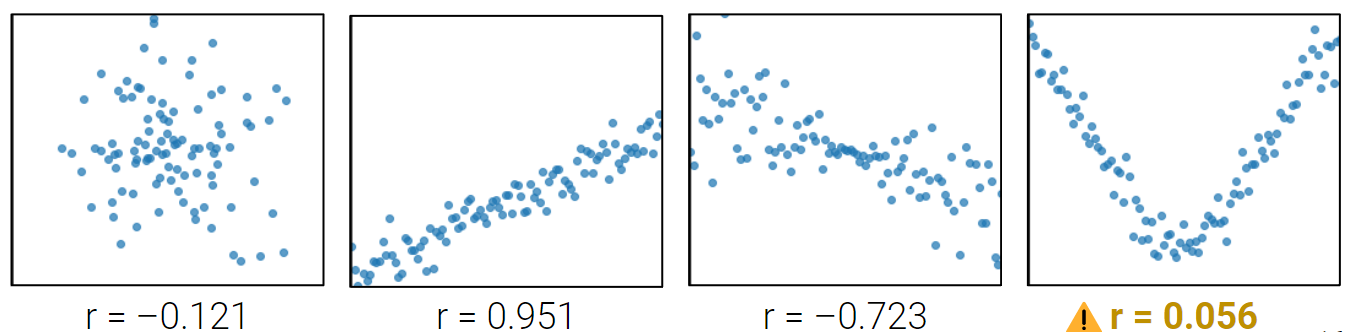
\includegraphics[scale=0.4]{figs/ln01/linear-correlation.png}
    \end{center}
\end{ln-define}

At this point, you will probably have the following concerns:
\begin{bindenum}
    \item What does it mean when a parameter is ``best'' or ``most accurate''?
    \item How do we obtain such parameters?
\end{bindenum}
And here is where we deal with the mathematics of regression lines.

\subsection{Model Selection: Simple Linear Regression}
The \textbf{Simple Linear Regression} model is essentially a model using the regression line to predict the $y$ of a datapoint for the $x$ of a datapoint. In most definition, it's bound to only produce a two-dimensional regression line. \\
Such a model's prediction relies entirely on the value of its parameters. We recognize this by saying that Simple Linear Regression is a \textbf{parametric model}, described by its parameters $a$ and $b$. \\
You might have noticed from the few graphs above that, the regression line doesn't accurately predict every single point. It is born from a set of points that don't necessarily form a line. Therefore, the best parameters that we provide it (again, called $\hat{a}$ and $\hat{b}$), are what we call the sample-based estimate of the inexistent, completely correct regression line. \\
Following that same logic, we noted the result of prediction as $\hat{y}$: our best estimate of the actual $y$ of a new, unseen datapoint.

\subsection{Quantifying Errors: Loss Functions}
To quantify how ``good'' a prediction is, we would like to use a loss function:
\begin{ln-define}{Loss Function}{}
    A \textbf{loss function} is a function that characterizes the cost in predictions for choosing a set of parameters. \\
    It quantifies how bad a prediction is for a single observation. The closer our prediction is to the actual observed value, the better the prediction, therefore, the lower the loss. Vice versa.
\end{ln-define}
The choice of loss function affcets how we customize our model to adapt to mistakes. While it affects the accuracy of estimations, it would also decide the computational cost of estimation, as some loss functions are very costly to calculate for computers. \\
For Simple Linear Regression, we usually bother with two choices of loss functions:
\begin{ln-define}[sidebyside]{Loss Functions of SLR}{}
    \textbf{Squared Loss} (L2 Loss) \\
    \[L(y, \hat{y}) = {(y - \hat{y})}^2\]
    This is a reasonable choice because there would be no loss when prediction is equal to observed value, and provide a lot of loss for predictions that are far from the observed values.
    \tcblower
    \textbf{Absolute Loss} (L1 Loss) \\
    \[L(y, \hat{y}) = |y - \hat{y}|\]
    This is a reasonable choice because there would be no loss when prediction is equal to observed value, and provide a fair amount of loss at a uniform sign (positive) for predictions that are far from the observed values (benefited from the absolute value).
\end{ln-define}
Since we concern how costly our model's predictions are for the entire data set, the natural measure of how good a model is would be the average loss of model across all data points. This is also known as \textbf{empirical risk}:
\begin{ln-define}{Empirical Risk}{}
    The empirical risk is the average loss of a model across all data points. Minimizing empirical risk provides the optimal estimated parameters of a model for the corresponding loss function. \\
    Mathematically expressed,
    \[\hat{R}(\theta) = \frac{1}{n} \sum_i L(y_i, \hat{y}_i)\]
    Here, $\theta$ represents the parameters of the model.
\end{ln-define}
Let us inspect the case where we attempt to minimize the empirical risk with our loss being L2 loss function. In this case, we call our empirical risk \textbf{Mean Squared Error}.
\begin{ln-derive}{Estimated Parameters of Simple Linear Regression under MSE}{}
    To recall:
    \[MSE(a, b) = \frac{1}{n} \sum_i {(y_i - a - b x_i)}^2\]
    To minimize this function, we will find the conditions where the partial derivative of $MSE$ with respect to every parameter is $0$. \\
    \textbf{Minimizing a}: \\
    \begin{align*}
        \pdv{MSE}{a} &= \frac{1}{n} \times \sum_i 2\frac{\delta}{\delta a}(y_i - a - b x_i)(y_i - a - b x_i) \\
        &= \frac{1}{n} \times \sum_i -2(y_i - a - b x_i) \\
        &= -\frac{2}{n} \sum_i (y_i - a - b x_i) \\
        \frac{1}{n} \sum_i (y_i - \hat{y}_i) &= 0 \\
        \sum_i (y_i - a - b x_i)
        &= \sum_i (y_i) - a - b\sum_i (x_i) \\
        &= \overline{y} - a - b \overline{x} = 0 \\
        a &= \overline{y} - b \overline{x}
    \end{align*}
    \textbf{Minimizing b}: \\
    \begin{align*}
        \pdv{MSE}{b} &= \frac{1}{n} \times \sum_i 2\frac{\delta}{\delta b}(y_i - a - b x_i)(y_i - a - b x_i) \\
        &= \frac{1}{n} \times \sum_i -2x_i(y_i - a - b x_i) \\
        &= -\frac{2}{n} \sum_i x_i(y_i - a - b x_i) \\
        \frac{1}{n} \sum_i x_i(y_i - \hat{y}_i) &= 0 \\
        \frac{1}{n} \sum_i x_i(y_i - \hat{y}_i) - \frac{1}{n} \sum_i \overline{x} (y_i - \hat{y}_i)
        &= \frac{1}{n} \sum_i (x_i - \overline{x}) (y_i - \hat{y}_i) \\
        &= \frac{1}{n} \sum_i (x_i - \overline{x}) (y_i - \overline{y} - b(x_i - \overline{x})) = 0 \\
        \frac{1}{n} \sum_i (x_i - \overline{x}) (y_i - \overline{y})
        &= b \frac{1}{n} \sum_i (x_i - \overline{x}) (x_i - \overline{x}) \\
        r_{x, y} \sigma_x \sigma_y &= b \sigma_x^2 \\
        b = r \frac{\sigma_y}{\sigma_x}
    \end{align*}
    \tcblower
    Conclusion:
    \[
        \begin{cases}
            \hat{a} = \overline{y} - \hat{b} \overline{x} \\
            \hat{b} = r \frac{\sigma_y}{\sigma_x}
        \end{cases}
    \]
\end{ln-derive}
So at last, we also find that the optimizing condition of SLR model would be:
\[
    \begin{cases}
        \frac{1}{n} \sum_i (y_i - \hat{y}_i) &= 0 \\
        \frac{1}{n} \sum_i x_i(y_i - \hat{y}_i) &= 0
    \end{cases}
\]
Which can be interpreted respectively as that:
\begin{bindenum}
    \item The residuals average to 0.
    \item The residuals are orthogonal to the predictor variable.
\end{bindenum}

\newpage
\chapter{DATA C100: Constant Model in Linear Regression}

\section{Defining the Constant Model}
Now that we have finished reading about simple linear regression from the previous lecture, let us discuss a slightly simpler model.
\begin{ln-define}{Constant Model}{}
    \textbf{Constant Model}, also known as a summary statistic, summarizes the sample data by always predicting the same number for any data point. \\
    Mathematically expressed,
    \[\hat{y} = \theta\]
\end{ln-define}
In other words, the estimated $y$ is always a constant parameter $\theta$, whatever the input might be.

\section{Experimenting Different Loss Functions}
A model may have several options for its loss functions, which comes with different advantages and disadvantages. \\
For this constant model, let us explore the L2 and L1 loss functions, see how each brings a different condition of optimization and robustness.

\subsection{Exploring L2 Loss: MSE}
In the L2 case, let us recall that our empirical risk is defined as follows:
\[R(\theta) = \frac{1}{n} \sum_{i = 1}^n {(y_i - \hat{y}_i)}^2\]
Therefore, for our constant model:
\[R(\theta) = \frac{1}{n} \sum_{i = 1}^n {(y_i - \theta)}^2\]
Let us proceed onto its optimization by attempting to find the critical point of empirical risk:
\begin{ln-derive}{Optimization of L2 Empirical Risk for Constant Model}{}
    Noting that the empirical risk can be expressed as:
    \[R(\theta) = \frac{1}{n} \sum_{i = 1}^n {(y_i - \theta)}^2\]
    We may perform the following derivation:
    \begin{align*}
        \pdv{R}{\theta}
        &= \frac{1}{n} \sum_{i = 1}^n 2\frac{\delta}{\delta \theta}(y_i - \theta){(y_i - \theta)} \\
        &= -\frac{2}{n} \sum_{i = 1}^n (y_i - \theta)
    \end{align*}
    And now, to optimize $R$,
    \begin{align*}
        \sum_{i = 1}^n (y_i - \theta) &= 0 \\
        \overline{y} - \theta &= 0 \\
        \theta = \overline{y}
    \end{align*}
    Therefore, 
    \[\hat{\theta} = \overline{y}\]
\end{ln-derive}
Let us enjoy some observations here. \\
First of all, the minimum MSE is thus:
\[R(\theta) = \frac{1}{n} \sum_{i = 1}^n {(y_i - \overline{y})}^2 = \sigma_y^2\]
, which is a statistic that we call the variance of $y$. \\
Second of all, the estimated value of parameter $\theta$ is thus the mean of $y$. This means, provided an extreme outlier, the model will misbehave due to the mean being heavily influenced by some extreme outlier(s). Therefore, L2 Loss is not very robust (adaptative) towards the appearance of outliers. \\
And from here, we will begin to recognize that many good or popular loss functions come with interesting mathematical properties.

\subsection{Exploring L1 Loss: MAE}
The L1 Loss Empirical Risk is also known as \textbf{Mean Absolute Difference}, which followed a similar naming logic to MSE. \\
\[R(\theta) = \frac{1}{n} \sum_{i = 1}^n |(y_i - \theta)|\]
The optimization of such an empirical risk becomes interesting (matheamtically), due to the appearance of absolute value. \\
However, we may always characterize the absolute value as a piecewise function:
\[
    f(x) = |x - \theta|
    \rightarrow
    f(x) = 
    \begin{cases}
        x - \theta, &x > \theta \\
        0, &x = \theta \\
        \theta - x, &x < \theta
    \end{cases}
\]
Let us exploit this in the following toil:
\begin{ln-derive}{Optimization of L1 Empirical Risk for Constant Model}{}
    \[
        |y_i - \theta|
         = 
        \begin{cases}
            y_i - \theta, &y_i > \theta \\
            0, &y_i = \theta \\
            \theta - y_i, &y_i < \theta
        \end{cases}
    \]
    \[
        \frac{\delta}{\delta \theta}|y_i - \theta|
        = 
        \begin{cases}
            1, &y_i > \theta \\
            0, &y_i = \theta \\
            -1, &y_i < \theta
        \end{cases}
    \]
    \begin{align*}
        \pdv{R}{\theta}
        &= \frac{1}{n} (\sum_{\theta < y_i}(-1) + \sum_{\theta > y_i}(1)) \\
        \sum_{\theta < y_i}(-1) + \sum_{\theta > y_i}(1) &= 0 \\
        \sum_{\theta > y_i}(1) = \sum_{\theta < y_i}(1)
    \end{align*}
    Therefore, $\hat{\theta}$ must be the median of $y$.
\end{ln-derive}
The estimated value of parameter $\theta$ is thus the mean of $y$. This means, provided an extreme outlier, the model will not misbehave due to the median not easily influenced by some extreme outlier(s). Therefore, L1 Loss is more robust (adaptative) towards the appearance of outliers. \\
Now, quoting the assignment of this course, we may also derive the optimal constant $\hat{\theta}$ on any similar piecewise linear cost functions; say:
\begin{ln-derive}{Optimization of Weighted L1 Empirical Risk for Constant Model}{}
    Let the residual function be noted as:
    \[
        L(y, \hat{y})
         = 
        \begin{cases}
            |y - \hat{y}|, &y > \hat{y} \\
            w|y - \hat{y}|, &y < \hat{y}
        \end{cases}
    \]
    from which we may differentiate the loss function with respect to $\hat{y} = \theta$, and acquire that:
    \[
        \pdv{L}{\theta}(y, \hat{y})
         = 
        \begin{cases}
            -1, &y > \hat{y} \\
            w, &y < \hat{y}
        \end{cases}
    \]
    Therefore, to optimize on this function:
    \[
        \sum_{y < \hat{y}}w - \sum_{y > \hat{y}} = 0
    \]
    And the value of $\hat{y}$ would have to be on the $\frac{1}{1 + w}$ quantile.
\end{ln-derive}

\subsection{Summary of Loss Function Optimization}
In summary, the process of finding optimization conditions (which we also call \textbf{estimating equation}) would follow:
\begin{enumerate}
    \item Differentiate the empirical risk with respect to parameters.
    \item Attempt to find the critical point of empirical risk for per parameter.
    \item Perform the derivative test (which requires multivariable calculus in most occassions, and is not performed for the span of DATA C100 for that reason) to confirm that the critical point is a minima.
\end{enumerate}
The multivariable perspective offers a much computationally heavy test for confirming whether a critical point is a minima, which would involve calculating plural higher order partial derivatives. For those who are interested, this is in-scope for MATH 53.

\section{Transformation and Model Linearity}
In some cases, we face how the predictor variable $x$ is not linearly correlated with $y$, but a transformation of $x$ might be. \\
For example, the trajectory of a baseball is mostly quadratic. If I'd like to predict its motion, it is best that I present a model whose shape is not linear, but rather, quadratic:
\[\hat{y} = \hat{a} + \hat{b} x^2 \]
This happens frequently across datasets, but the question is: is the model still linear in this case? \\
The answer is yes. \\
Linear Regression requires a regression line, decided as a linear combination of parameters. In this case, the predictor variable is being a non-linear term, but the regression equation is still linear with respect to each of the parameters.

As previously mentioned, models sometimes require transformations to behave better, fitting to the behaviour of the dataset more closely. \\
To decide what transformations seem optimal, we can employ the following figure:
\begin{ln-fig}{Turkey-Mosteller Bulging Diagram}{}
    \begin{center}
        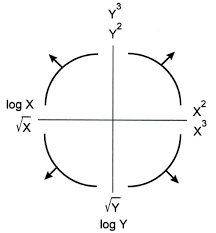
\includegraphics[scale=0.6]{figs/ln02/turkey-mosteller.png}
    \end{center}
\end{ln-fig}
Each of these transformations suggest how to transform $x$ and $y$ via suggesting that, for the direction that data's shape currently bulges towards, we should transform $x$ and/or $y$ in that direction. \\
In this case, we are usually then given the choice to either transform $x$ or $y$, or as priorly mentioned, perhaps both.

\newpage
\chapter{DATA C100: Ordinary Least Squares}

\section{Multiple Linear Regression Model}
We have seen Simple Linear Regression Model, which uses one parameter for a constant term and another parameter to introduce the predictor variable. \\
The model currently has one predictor variable. \\
What if we can use more? What if we need to use more? What if our model would benefit greatly because what we attempt to predict in nature requires two or more variables for a good prediction? \\
If so, such a model would have some regression equation whose shape is to a huge degree similarly shaped as below:
\[\hat{y} = \theta_0 + \theta_1 x_1 + \theta_2 x_2 + \cdots + \theta_p x_p\]
Let us attempt to vectorize the above equation. Suppose, we rewrite the above equation as follows:
\[
    \hat{y}^{(i)} = 
    \begin{bmatrix} 1 & x_1^{(i)} & \cdots & x_p^{(i)} \end{bmatrix}
    \begin{bmatrix} \theta_0 \\ \vdots \\ \theta_p \end{bmatrix}
\]
Then, we have successfully written the above equation in a matrix-vector multiplication form. \\
The anatomy of each term in the above row vector, $x_k^{(i)}$, is as follows:
\begin{bindenum}
    \item $x^{(i)}$ stands for the $i^{th}$ data point inside the dataset.
    \item $x_k$ stands for the $k^{th}$ feature inside the dataset.
    \item Therefore, $x_k^{(i)}$ is the $k^{th}$ feature of $i^{th}$ data point inside the dataset.
    \item Among all columns, we appended another column of ones on the left of row vector to account for the need of intercept in regression line.
\end{bindenum}
To vectorize this operation across numerous datapoints in the dataset, we may then formulate this model in terms of matrix-vector multiplication as follows:
\[
    \begin{bmatrix} \hat{y}_1 \\ \vdots \\ \hat{y}_k \end{bmatrix} =
    \begin{bmatrix} 
        1 & x_1^{(1)} & \cdots & x_p^{(1)} \\
        \vdots & \vdots & \vdots & \vdots \\
        1 & x_1^{(k)} & \cdots & x_p^{(k)}
    \end{bmatrix}
    \begin{bmatrix} \theta_0 \\ \vdots \\ \theta_p \end{bmatrix}
\]
And each term can then be respectively abbreviated into what is shown below:
\[\Y = \X \theta\]
Where we specifically name the matrix $\X$ containing the datapoints as the \textbf{design matrix}.

\section{Optimization of Model: Least Squares Algorithm}

\subsection{Loss Function}
The Loss function most frequently applied for such a model has to deal with a linear algebraic property called L2 Norm:
\begin{ln-define}{L2 Norm}{}
    The L2 Norm of a vector $\vec{x} \in \R^n$ is mathematically expressed as:
    \[{||x||}_2 = \sqrt{\sum_{i = 1}^n x_i^2}\]
    which occurs to be the magnitude of such vector $\vec{x}$. \\
    We thus notate the distance of vectors $\vec{a}, \vec{b} \in \R^n$ as:
    \[{||a - b||}_2\]
\end{ln-define}
Our L2 loss function would be the distance between estimation and observed values, squared:
\[{||\Y - \hat{\Y}||}_2^2\]
Therefore yielding the empirical risk:
\[R(\theta) = \frac{1}{n} {||\Y - \X \theta||}_2^2\]

\subsection{Optimization via Geometric Interpretation}
We should first observe with our prior knowledge from EECS 16A (or alternatively MATH 54, just any college linear algebra introductory course), that since $\hat{Y}$ is a linear combination of the columns of $\X$ (as noted $\hat{Y} = \X \theta$),
\[\hat{\Y} \in span(\X) \subseteq \R^k\]
However, it is not necessary that $\Y$ belongs to the span of $\X$. Therefore, we see more clearly that our task is to minimize the distance between $\Y \notin span(\X)$ and $\hat{\Y} \in span(\X)$. \\
Let us observe a visualization from the DATA C100 Lecture Slides (since mine are underqualified and old):
\begin{ln-fig}{Geometric Image of Residual in Multiple Linear Regression}{}
    \begin{center}
        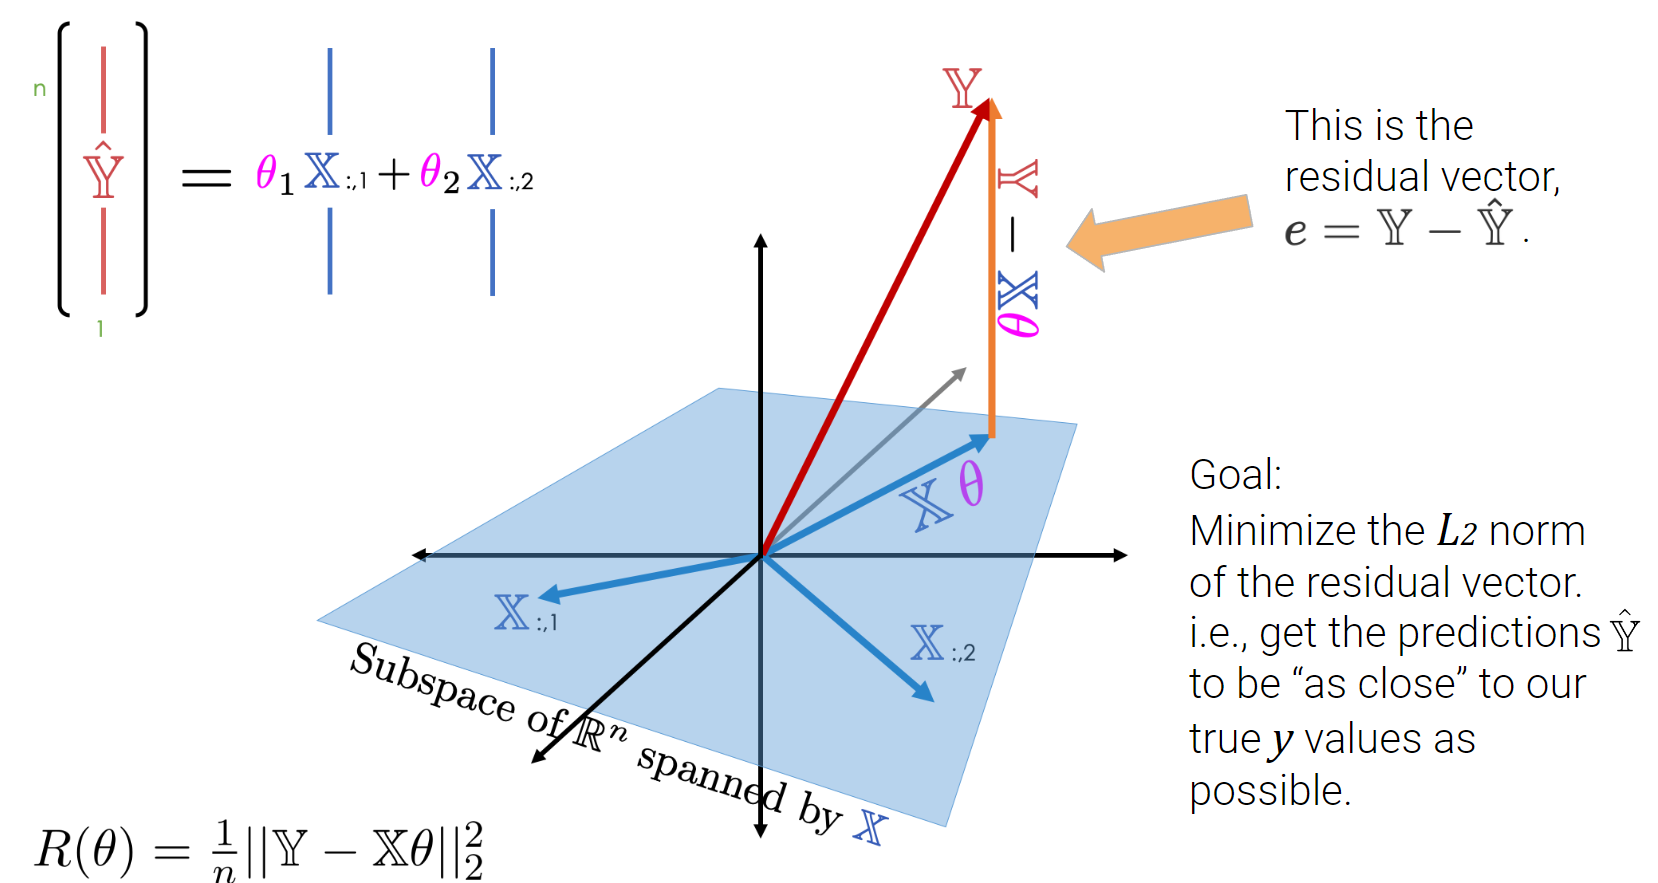
\includegraphics[scale=0.3]{figs/ln03/least-square-geometry.png}
    \end{center}
\end{ln-fig}
This residual vector is essentially the shortest possible (minimized) when it is orthogonal to $\X \theta$ (which, in a 2D view, has to do with a property of right triangles called the Pythagorean Theorem). \\
There is a better intuition than Pythagorean Theorem, which is that the vector in $span(\X)$ closest to $\Y$ must be its projection onto $span(\X)$. \\
Either way, we will be introduced to a simplified situation:
\begin{quote}
    To minimize 
    \[R(\theta) = \frac{1}{n} {||\Y - \X \theta||}_2^2\]
    We require that
    \[\X^T (\Y - \X \hat{\theta}) = 0\]
    Such that the residual is orthogonal to $span(\X)$.
\end{quote}
Let us review its solution from EECS 16AB (or MATH 54, MATH 110):
\begin{ln-derive}{Least Squares Algorithm}{}
    \begin{align*}
        \X^T (\Y - \X \hat{\theta}) &= 0 \\
        \X^T\Y &= \X^T\X \hat{\theta} \\
        \hat{\theta} &= {(\X^T\X)}^{-1} \X^T\Y
    \end{align*}
\end{ln-derive}
The equation above that shows the optimal parameters is known as the \textbf{Normal Equation}. \\
This normal equation would only be useful when $\X^T \X$ is invertible. Determining whether $\X^T \X$ is invertible is not as difficult as it sounds, since $N(A^T A) = N(A)$. I will not showcase this proof here. \\
Beyond the scope of DATA C100, we should also see some remedy for such situations when attempting to solve this exact optimization problem and working with a non-invertible design matrix. It is also not in the scope of this note yet.

\section{Performance Factors}
Just like in previous models, the residuals should be uncorrelated with the predicted values $\hat{y}$. \\
To determine the correlation of variables in a multivariable perspective like in Multiple Linear Regression, we work with a new coefficient:
\begin{ln-define}{Coefficient of Determination}{}
    The coefficient of determination characterizes the correlation of variables in a Multiple Linear Regression model:
    \[R^2 = \frac{\text{Variance of predicted values}}{\text{Variance of observed values}} = \frac{\sigma_{\hat{y}}^2}{\sigma_y^2}\]
\end{ln-define}
Just like the Pearson's Correlation Coefficient ($r$ in Simple Linear Regression), $R^2$ spans between $0$ and $1$ (except it is the absolute value of $r$ that spans between $0$ and $1$, not $r$ itself).

\newpage
\chapter{DATA C100: Gradient Descent}

\section{Computational Minimization of Loss Function}
We have been able to minimize the loss functions provided for prior linear regression models. But we may always encounter harder loss functions to analyze, either via calculus or linear algebra-geometry. \\
This is where we fall back to the power of computation. Numerical computing. Such subfield of computer science focuses on solving complex mathematical problems using arithmetic operations. Very fortunately, Python is well supported by such libraries:
\setbox\codebox=\hbox{
    \begin{lstlisting}
    scipy.optimize.minimize
    Args:
        fun: The objective function to be minimized, where $x$ is a 1D
        array.
        x0: Initial guess, with the same size as input x from fun.
    Returns:
        The result of optimization with a solution array for optimal
        parameters.
    Example:
        >>> from scipy.optimize import minimize
        >>> minimize(arbitrary, x0 = [6, 3])
        OptimizationResult(x = [5.5, 2])
    \end{lstlisting}
}
\begin{ln-code}{Using scipy to Minimize Functions}{}
    \usebox\codebox
\end{ln-code}

\section{Gradient Descent Algorithm}
When in a multivariable context, the loss function might take plural inputs and thus not be plottable in the two-dimensional space anymore. In that case, each point $(x_1, x_2)$ correspond to the cost of choosing them as model parameters, and we end up with a loss surface.
\begin{ln-fig}{Loss Function as a Surface}{}
    \begin{center}
        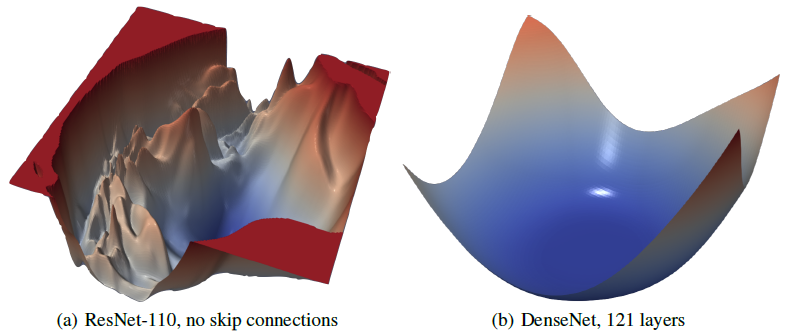
\includegraphics[scale=0.4]{figs/ln04/loss-surface.png}
    \end{center}
    As you may see, each point $(x_1, x_2)$ has a respective height for their respective loss value. Therefore, the lowest point on the surface is the point of optimization, where by choosing that point as the set of parameters, we arrive at the lowest possible loss value. \\
    We will also take notice on why the right-side surface is much preferrable than the left-side surface.
\end{ln-fig}
Now, our task is focused on ``how to descend on the loss surface''. The entire algorithm that breifly leads us to descend off the loss surface is therefore known as the Gradient Descent Algorithm.

\subsection{Interpretation of Gradients}
This section is noted from MATH 53. It is not in scope for DATA C100. However, I think the reader can benefit from knowing what gradients are. \\
Let us begin with the notion of Directional Derivatives:
\begin{ln-define}{Directional Derivatives}{}
    We know how to compute the partial derivatives for a function $f(x, y)$ with respect to $x$ and $y$, which are respectively the rate of change of $f$ as we solely vary $x$ and solely vary $y$. \\
    The \textbf{directional derivative}, then, is the rate of change of $f$ when we let both variables $x$ and $y$ change. Mathematically, we would be able to characterize the direction of changing as a vector. \\
    The rate of change of $f(x, y)$ along a unit vector $\vec{u} = <a, b>$ can thus be denoted as:
    \[D_{\vec{u}}f(x, y) = \lim_{h \rightarrow 0} \frac{f(x + ah, y + bh) - f(x, y)}{h}\]
    In practical form, after a series of derivations:
    \[D_{\vec{u}}f(x, y) = <f_x (x, y), f_y (x, y)> \cdot \vec{u}\]
\end{ln-define}
Recall that:
\[\cos(\theta_{\vec{u}, \vec{v}}) = \frac{\vec{u} \cdot \vec{v}}{|\vec{u}| |\vec{v}|}\]
Therefore, the directional derivative is maximized when the direction at which we change $x$ and $y$ is exactly the vector $<f_x (x, y), f_y (x, y)>$. \\
This means the direction provides the most positive change (provides the maximal rate of change) towards $f$, if we were to travel in that direction. For convenience and mathematical property, let us name this great observation as follows:
\begin{ln-define}{Gradient}{}
    The \textbf{gradient} of a function $f(x_1, \cdots, x_n)$ is the vector:
    \[\nabla f = \begin{bmatrix} \pdv{f}{x_1} \\ \cdots \\ \pdv{f}{x_n} \end{bmatrix}\]
    Where $\nabla f(x_1, \cdots, x_n)$ notes the direction of greatest ascent (greatest rate of value increase) along the function $f$ from $(x_1, \cdots, x_n)$
\end{ln-define}
In other words, the opposite direction of the gradient is the direction of greatest descent. We can thus come up with the following iterative procedure for descending along a loss surface of $f(x, y)$:
\setbox\codebox=\hbox{
    \begin{lstlisting}
    initial_guess = ? #an array of parameters for initial guess
    for _ in range(epoch):
        grad = gradient(f, x, y)
        initial_guess -= grad
    return initial_guess
    \end{lstlisting}
}
\begin{ln-code}{Sketch of Gradient Descent Algorithm}{}
    \usebox\codebox
\end{ln-code}

\subsection{Improving the Gradient Descent Sketch}
We have a few problems left. \\
First of all:
\begin{center}
    What if the direction of greatest descent doesn't lead us down anymore?
\end{center}
For example:
\begin{ln-fig}[sidebyside]{Divergence of Gradient Descent}{}
    \begin{center}
        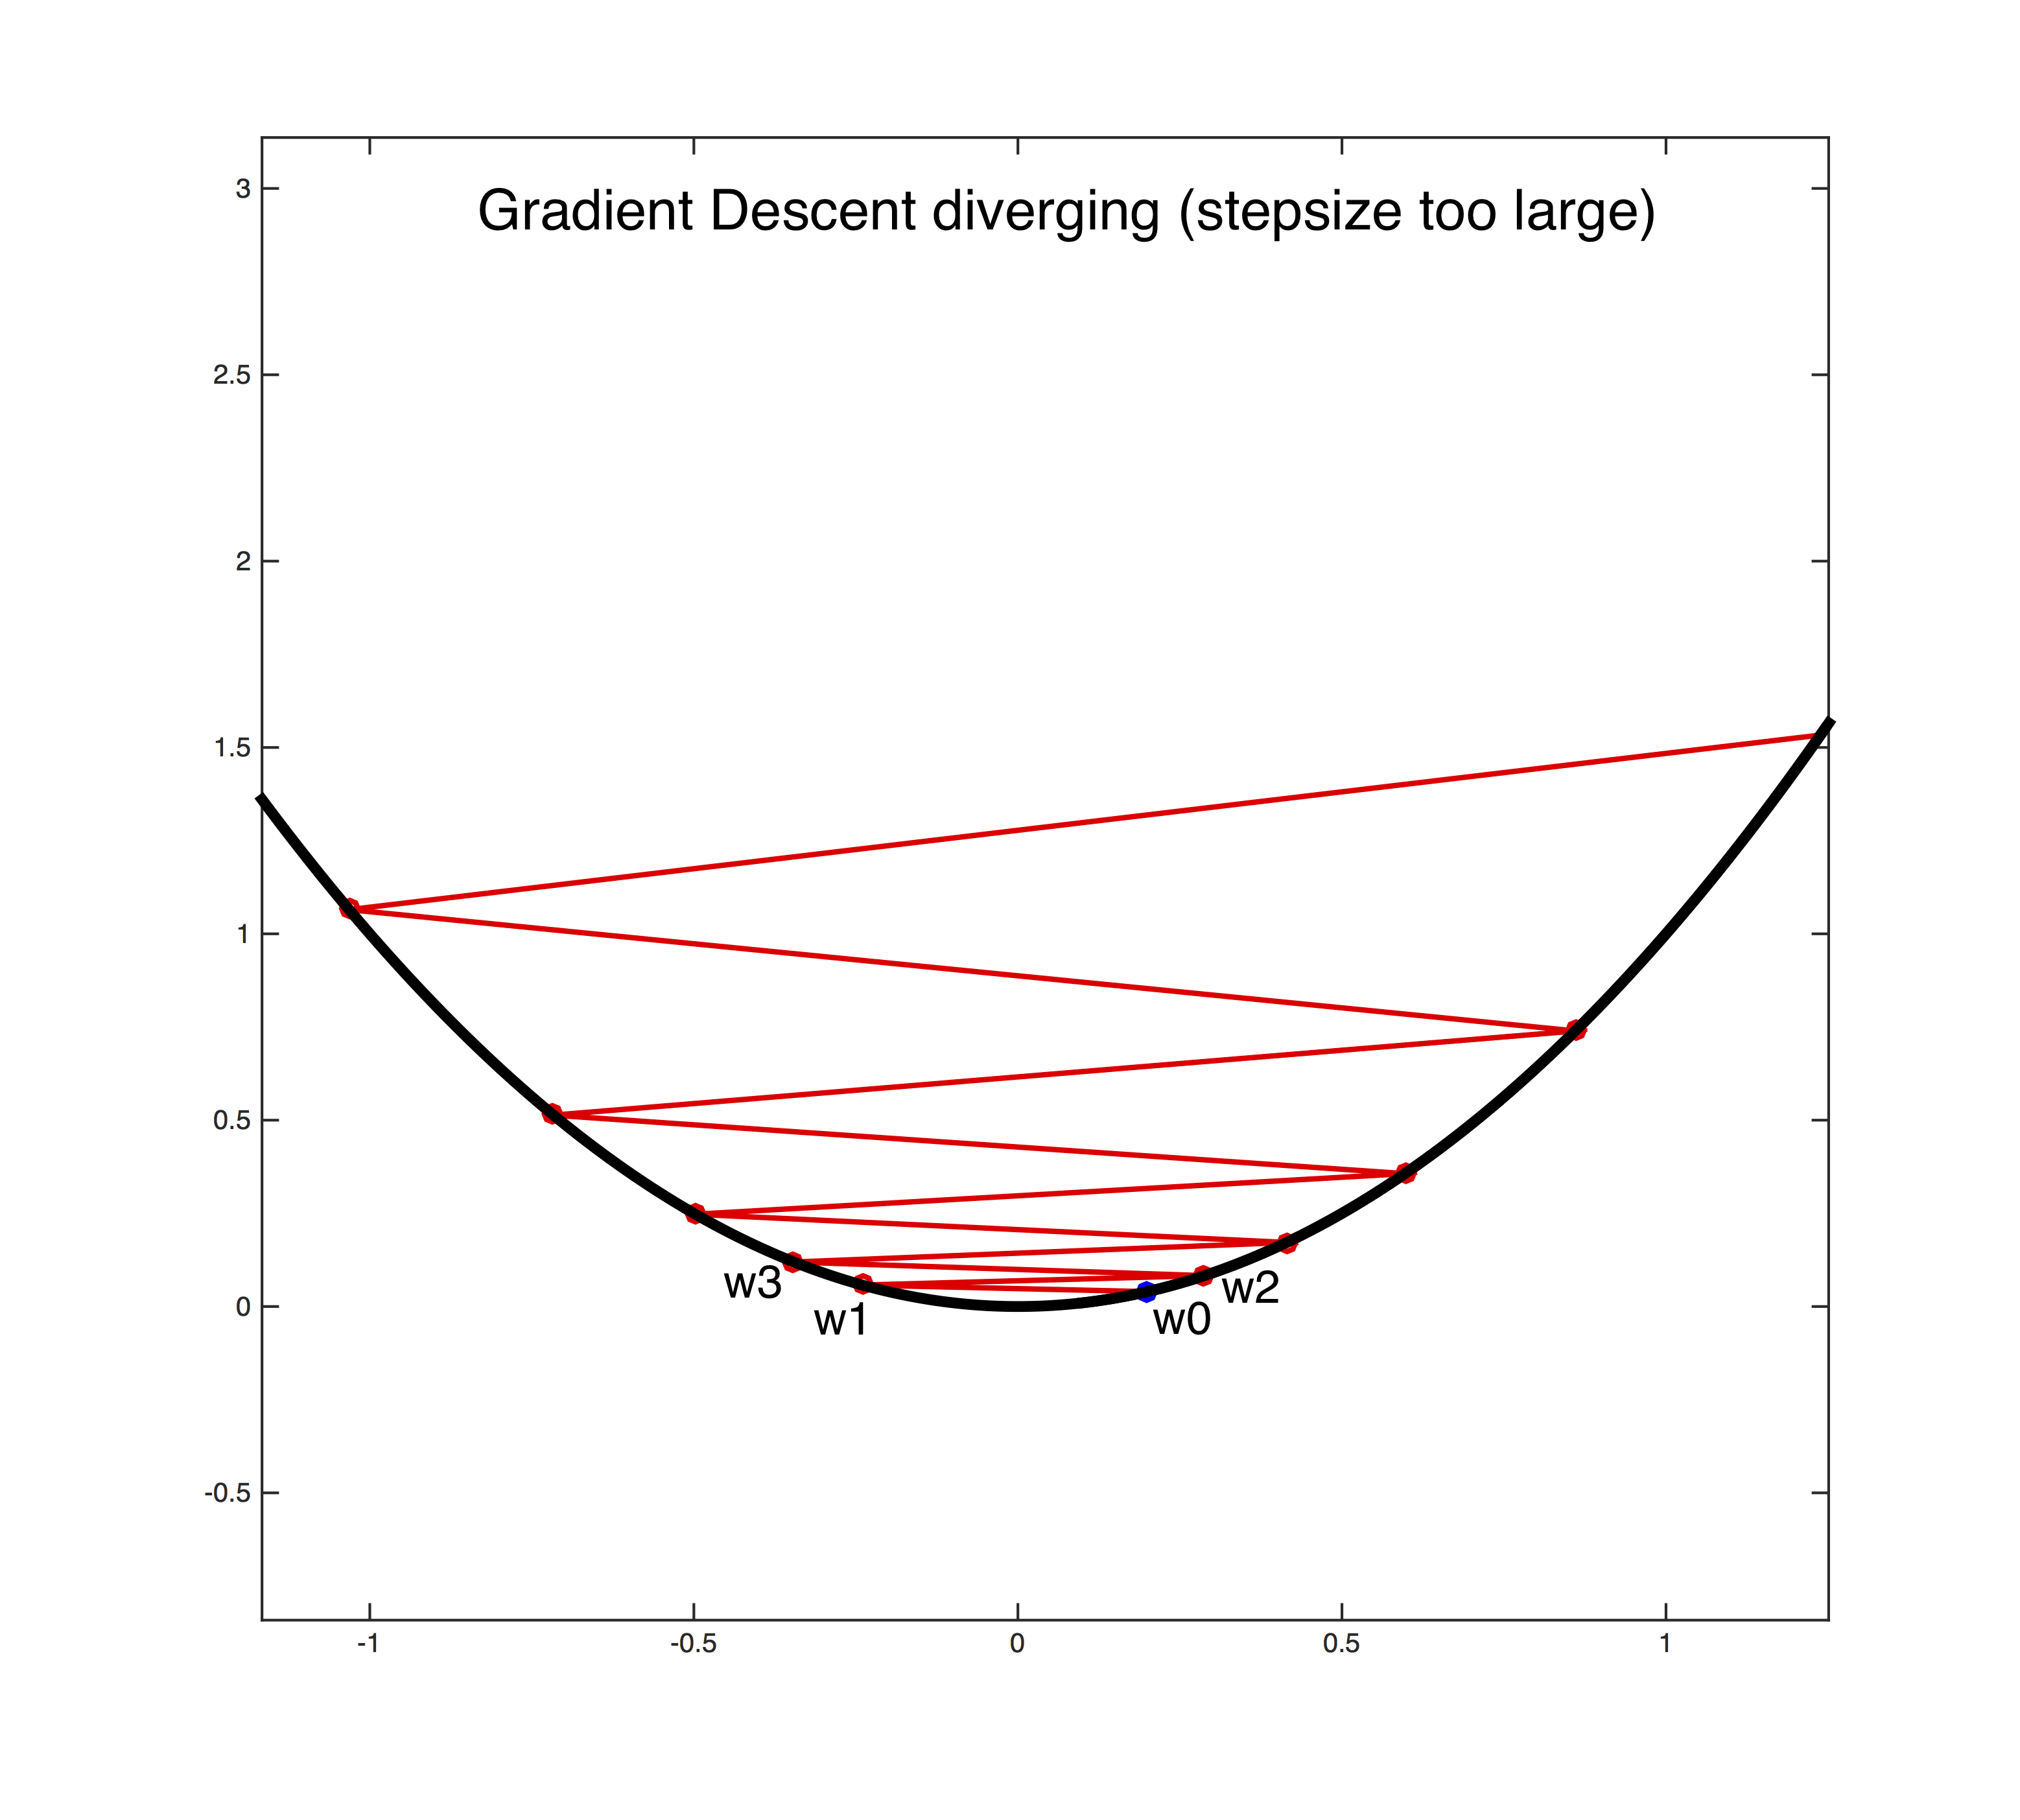
\includegraphics[scale=0.3]{figs/ln04/grad-descent-diverge.png}
    \end{center}
    \tcblower
    As you may see, because the gradient's magnitude is too big, we ended up going away from the local minima. \\
    To correct this situation, we will now improve the sketch of gradient algorithm to involve a parameter that controls what portion of the gradient do we travel. We call this the \textbf{learning step} ($\alpha$).
\end{ln-fig}
However, notice that if the learning step is small, then the distance at which we descent along the loss surface would also be smaller per iteration. This makes it take too long for gradient descent to converge at the minimum. 
Therefore, we would usually need to try learning steps by increasing or decreasing it tenfold until we find the appropriate learning step, and perhaps make it smaller as we go onto further iterations:
\setbox\codebox=\hbox{
    \begin{lstlisting}
    alpha = ? $customized learning step
    initial_guess = ? #an array of parameters for initial guess
    for _ in range(epoch):
        grad = gradient(f, x, y)
        initial_guess -= alpha * grad
    return initial_guess
    \end{lstlisting}
}
\begin{ln-code}{Gradient Descent Algorithm}{}
    \usebox\codebox
    Mathematically Expressed as a state-transition system (borrowing the work of EECS 16A):
    \[\vec{\theta}[t + 1] = \vec{\theta}[t] - a \nabla L(\vec{\theta}, x_1, \cdots, x_n)\]
\end{ln-code}

\subsection{Convexity}
We still have not decided how to make an initial guess of parameters, as well as how does gradient descent behave in real life. \\
First of all, let's perform a thought experiment. Suppose our loss function is a curve along which we gradient descent, what happens when we set the initial guess to the left side of the curve, and what happens when we guess from the right side of the curve instead?
\begin{ln-fig}[]{Loss Functions with Local Minima}{}
    \begin{center}
        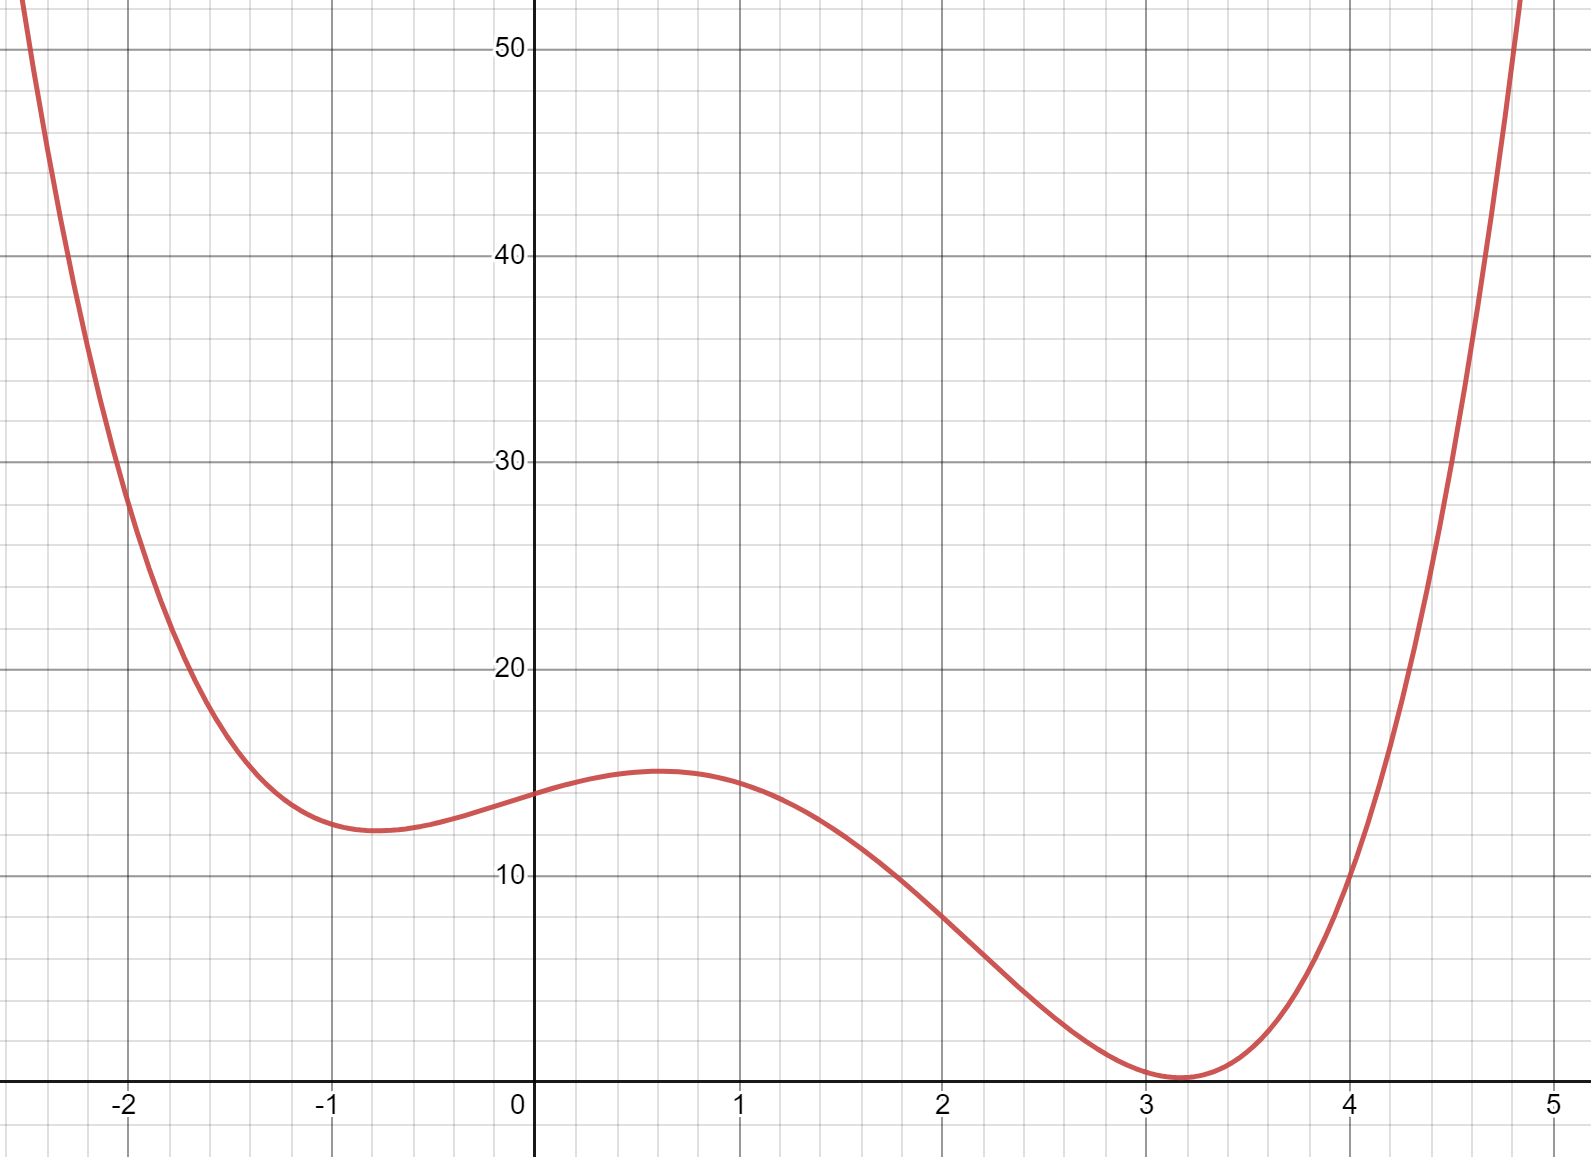
\includegraphics[scale=0.3]{figs/ln04/several-local-min.png}
    \end{center}
\end{ln-fig}
In this case, guessing from different directions would lead us to different local minima. Therefore, it is not exactly guaranteed that gradient descent leads us to the global minimum of our loss surface. \\
Then, if we manage to compromise with that (which we would have to, for now), how do we initialize our guess? This is where the idea of random initialization comes in for more complex models, where, we initialize each parameter to a random number as our initial guess. \\
For the scope of DATA C100, we would stick with zero initialization, where the initial guess of parameters would all be $0$. This would lead to a problem. If the gradient descent updates unfortunately lead to the parameters keep being equal, then we will realistically make no improvements on the model since every predictor variable receives the same weight in a regression equation. But, for now, let us not worry about this until a long time later.

But some functions guarantee us to find a global minimum when using gradient descent. These functions are called \textbf{convex functions}:
\begin{ln-define}{Convexity}{}
    Function $f$ is convex iff:
    \[\forall a, b \in D_f, t \in [0, 1] (tf(a) + (1 - t)f(b) \geq f(ta + (1 - t)b))\]
    Or in English: if a line is drawn between two points on the curve, all values on the curve must be on or below the line.
\end{ln-define}

\subsection{Stochastic Gradient Descent}
Sometimes, our dataset is too big. We would therefore need to perform gradient descent by batches:
\begin{ln-define}{Mini-Batch Gradient Descent}{}
    In mini-batch gradient descent, we use a subset of data to calculate the gradient. \\
    An approximate sketch of procedure follows:
    \begin{bindenum}
        \item Decide a batch size (The amount of data used to compute gradient). A popular choice is 32 (according to professor, for no particular reason it seems).
        \item For all batches:
        \subitem Compute gradient on current batch of the data
        \item Repeat the process until we arrive at a stopping condition where we decide we have optimized the parameters sufficiently.
    \end{bindenum}
\end{ln-define}
Via mini-batch gradient descent, we avoid heavy computational costs for large datasets and in turn are provided an approximation of the best way down an approximately true loss surface. It works well enough in practice.

We can also choose a batch size of $1$, which would be a process called \textbf{Stochastic Gradient Descent} (SGD in some libraries). \\
In this case, we compute gradient based on one single data point. This technique is used on datasets whose data entries involve many parameters, as via one datapoint, we may have updated millions of parameters for that epoch. In the long run, the effect of SGD is very similar to computing the true gradient based on the entire dataset. Therefore, it is also a practice-able choice for real-life machine learning models.

\newpage
\chapter{DATA C100: Feature Engineering}

\section{Motivation}
Lorem Ipsum.

\section{One Hot Encoding}
Lorem Ipsum.

\newpage
\chapter{DATA C100: Cross Validation}

\section{Variance and Training Error}
When attempting to form a model for predicting new datapoints, say linear regression, we often have some way to find optimal parameters. \\
The process of finding these parameters that lead to the best predictions possible is known as \textbf{training}. However, even the model itself would then have some errors when compared to the original data. This error is known as the \textbf{training error}. \\
To reduce training error, we might sometimes make the model more complex, so it covers more ground by using more information from a data entry and can end up making better predictions. The sensitivity of our model towards its fata is known as \textbf{variance}. \\
Of course, we can try to make a model entirely correct when applied onto the data we train it on. For an $n$-point dataset, we can use a $n-1$ degree polynomial that passes through all $n$ points of the dataset. At that point, the model has high variance, high complexity, and virtually $0$ training error. \\
But then, is this model use-able on other real-world data whose behavior deviates from the dataset?

Machine Learning scientists have developed the following famous diagram to discuss such phenomenon:
\begin{ln-fig}{Variance-Training Error Tradeoff}{}
    \begin{center}
        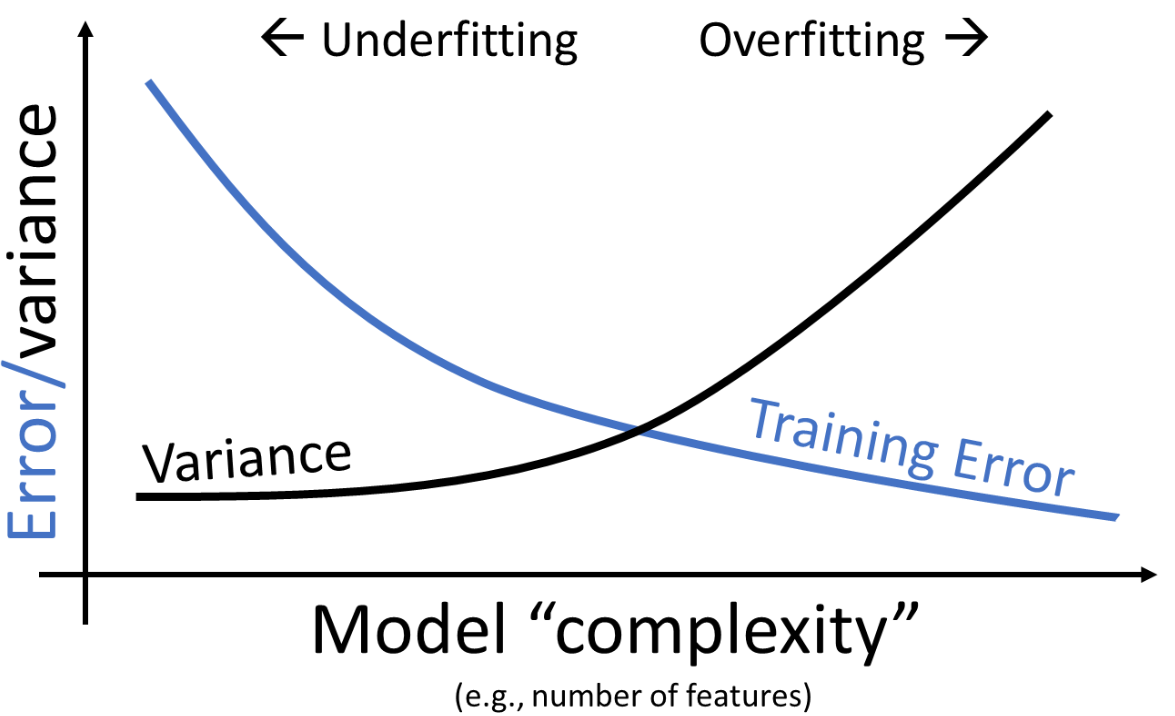
\includegraphics[scale=0.4]{figs/ln06/var-train-err-tradeoff.png}
    \end{center}
\end{ln-fig}

When a model \textbf{overfits}, it refers to the phenomenon discussed above: the model is aggressively tailored towards the dataset and fails to predict data outside the dataset it's trained on. \\
In this case, while we do attain a zero MSE, the model is useless outside the dataset we have trained on.

\section{Validation}
Scientists then came up with an idea: what if we attempt to validate our model using extra data point? \\
The first brief method that came into mind is a ``holdout method'', where for a datset of 100 points, we use 70 of 100 on training the data, which we call the \textbf{training set} (as in the dataset on which we train the model), and hold 30 of it out. \\
After training the dataset on the 70 data points, we test our model on the rest 30 which we have not trained on. This set of held out data is often called the \textbf{validation set} (or alternatively, development set, ``dev set''). \\
This allows us to validate our model by seeing how it behaves when predicting data outside the dataset we trained the model on. For the technology in DATA C100, its computation is as follows:
\setbox\codebox=\hbox{
    \begin{lstlisting}
    >>> from sklearn.utils import shuffle
    >>> training_set, dev_set = np.split(shuffle(df), [70])
    \end{lstlisting}
}
\begin{ln-code}{Hold-Out Dataset in Python}{}
    \usebox\codebox
\end{ln-code}
Ideally, we then arrive at what the following diagram describes:
\begin{ln-fig}{Variance-Erroe Tradeoff}{}
    \begin{center}
        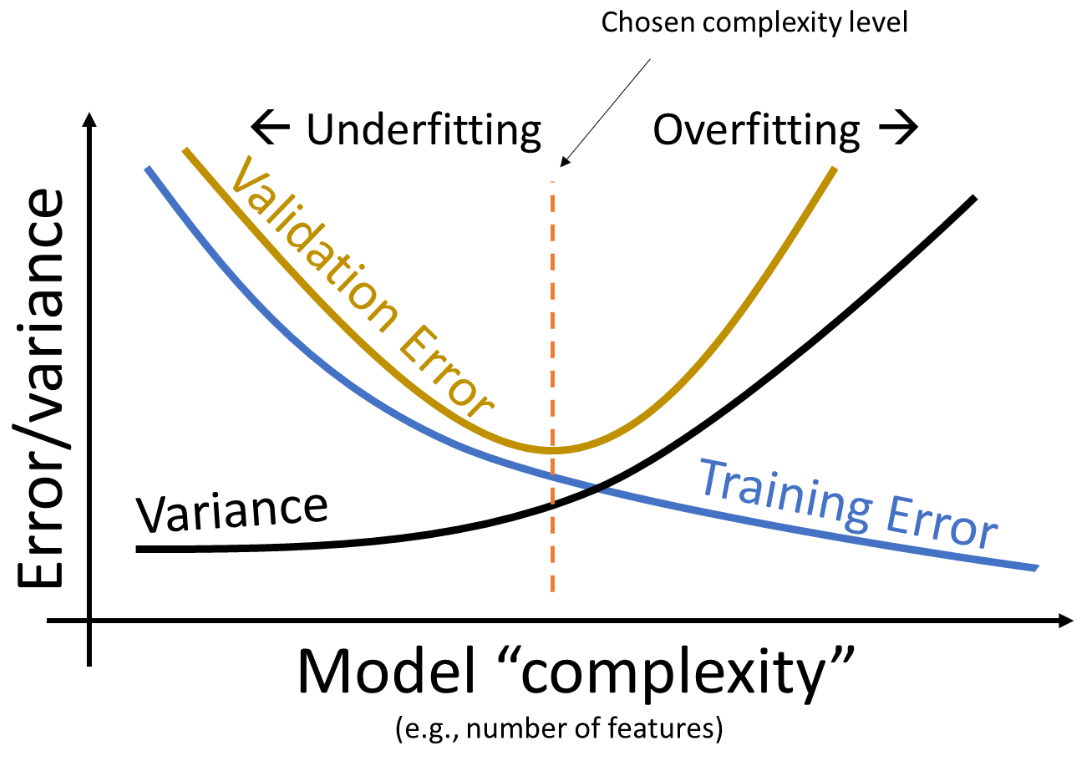
\includegraphics[scale=0.4]{figs/ln06/var-err-tradeoff.png}
    \end{center}
\end{ln-fig}
where we attempt to use a model whose complexity allows the minimum training error and validation error.

In this case, the degree of predictor variables, which form a polynomial for the regression line, is what we can blame and adjust for the deficiency of our model in overfitting. 
In machine learning, these variables that influence the learning process as outlined by the above tradeoff diagram is called \textbf{hyperparameter}. This can also involve, for example, the ratio of number of data in training set to that in validation set.

There is also an inherent problem with this hold-out idea, which we will address in the following section.

\section{K-Fold Cross Validation}
If we continue to use the same validation set for every single time we test our data, then our data would also be tailored towards the validation set. This causes a similar mistake to overfitting. \\
To address this issue, let us consider another similar approach of valiation, called \textbf{K-Fold Cross Validation}.

Imagine that we have divided our entire dataset into $k$ equal partition:
\begin{ln-fig}{K-Fold Cross Validation Sets}{}
    \begin{center}
        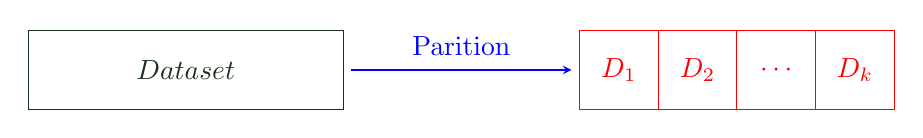
\begin{tikzpicture}
            \draw[green!10!black!90!]
                (0, 0) rectangle (4, 1)
                (2, 0.5) node{$Dataset$};
            \draw[blue]
                [-stealth](4.1, 0.5) -- (6.9, 0.5);
            \draw[blue]
                (5.5, 0.8) node{Parition};
            \draw[red]
                (7, 0) rectangle (8, 1)
                (7.5, 0.5) node{$D_1$}
                (8, 0) rectangle (9, 1)
                (8.5, 0.5) node{$D_2$}
                (9, 0) rectangle (10, 1)
                (9.5, 0.5) node{$\cdots$}
                (10, 0) rectangle (11, 1)
                (10.5, 0.5) node{$D_k$};
        \end{tikzpicture}
    \end{center}
\end{ln-fig}
Then, for each $i \in \{1, \cdots, k\}$, let us use the partition of dataset $D_i$ as our validation set to train the model. Denote the resulting validation error as ${VE}_i$. \\
Record such value from ${VE}_1$ to ${VE}_k$, and note the average of these validation errors as the overall validation error of training this model. \\
This way, we managed to validate our model without being stuck with one same validation set, and can provide a much more objective review towards the quality of current model complexity.

Popular choices of such value $k$ would be $5$, $10$, and $N$ (the length of the entire dataset). \\
In the case we have chosen to perform $N$-fold cross validation, which is also known as ``leave one out cross validation'', each point becomes a validation set and will usually yield the greatest result.
However, it is computationally expensive. \\
On the other hand, using $k = 5$ offers a less ideal result in tradeoff with a smaller computational cost.
\setbox\codebox=\hbox{
    \begin{lstlisting}
    GridSearchCV
    Args:
        estimator: The model for finding optimal parameters.
        param_grid: Hyperparameters stored in a dictionary.
        scoring: The loss function by which we assess performance
        of hyperparameters, usually "neg_mean_squared_error"
        cv: number of folds, or a 2D list containing indices
        for training set and dev set.
    Returns:
        The optimal parameters for estimator specified.
    \end{lstlisting}
}
\begin{ln-code}{Hold-Out Dataset in Python}{}
    \usebox\codebox
\end{ln-code}

\section{Test Set}
While we may find the model with the best validation set loss as the optimal one we will use in real life, when reporting the model on a public occassion (say paper, or actual incorporation with some procedure), we would like to assess our model using a special test set that we have never seen or used for any purpose. \\
This also relates back to how we preferred cross validation over hold-out on most occassions: avoiding biases towards the validation set used. \\
A test set can be easily produced via partitioning our original dataset into the \textbf{Training Set}, \textbf{Validation Set}, and \textbf{Testing Set}. We usually have some habits in how to partition a dataset into these subsets, such as producing a 70-15-15 partition.

To incorporate testing set into the big-picture of learning process with error-variance tradeoff, let's referrence this visual from DATA C100:
\begin{ln-fig}{Variance-Training Error Tradeoff}{}
    \begin{center}
        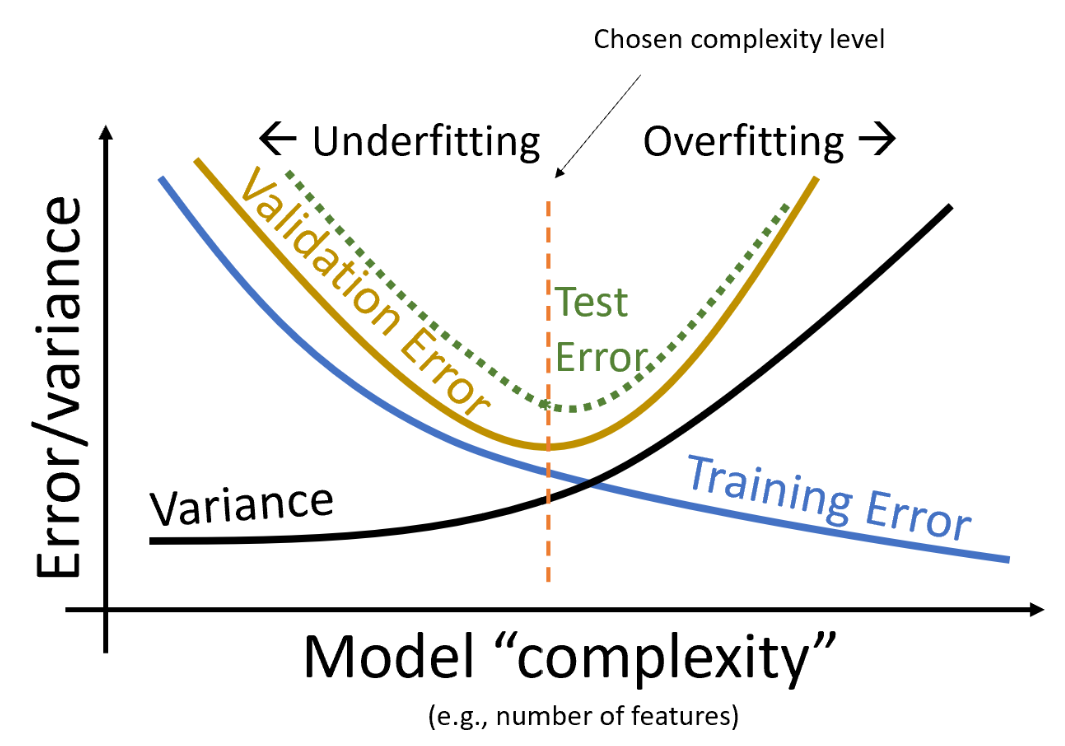
\includegraphics[scale=0.4]{figs/ln06/var-test-err-tradeoff.png}
    \end{center}
\end{ln-fig}
We may see that the only difference between testing error and validation error is essentially how restrictive the computation of those error is, as we are, for testing purposes, neither allowed nor supposed to access the error curve for testing set.

\newpage
\chapter{DATA C100: Regularization}

\section{General Introduction to Regularization}
There are other ways to prevent overfitting, and regularization is one of them. \\
The brief idea of regularization is to restrain the development on size of parameters. \\
For now, let us borrow a view from some two-parameter model under the gradient descent scheme for optimization:
\begin{ln-fig}{Regularization on Graphical Representation, DATA C100}{}
    \begin{center}
        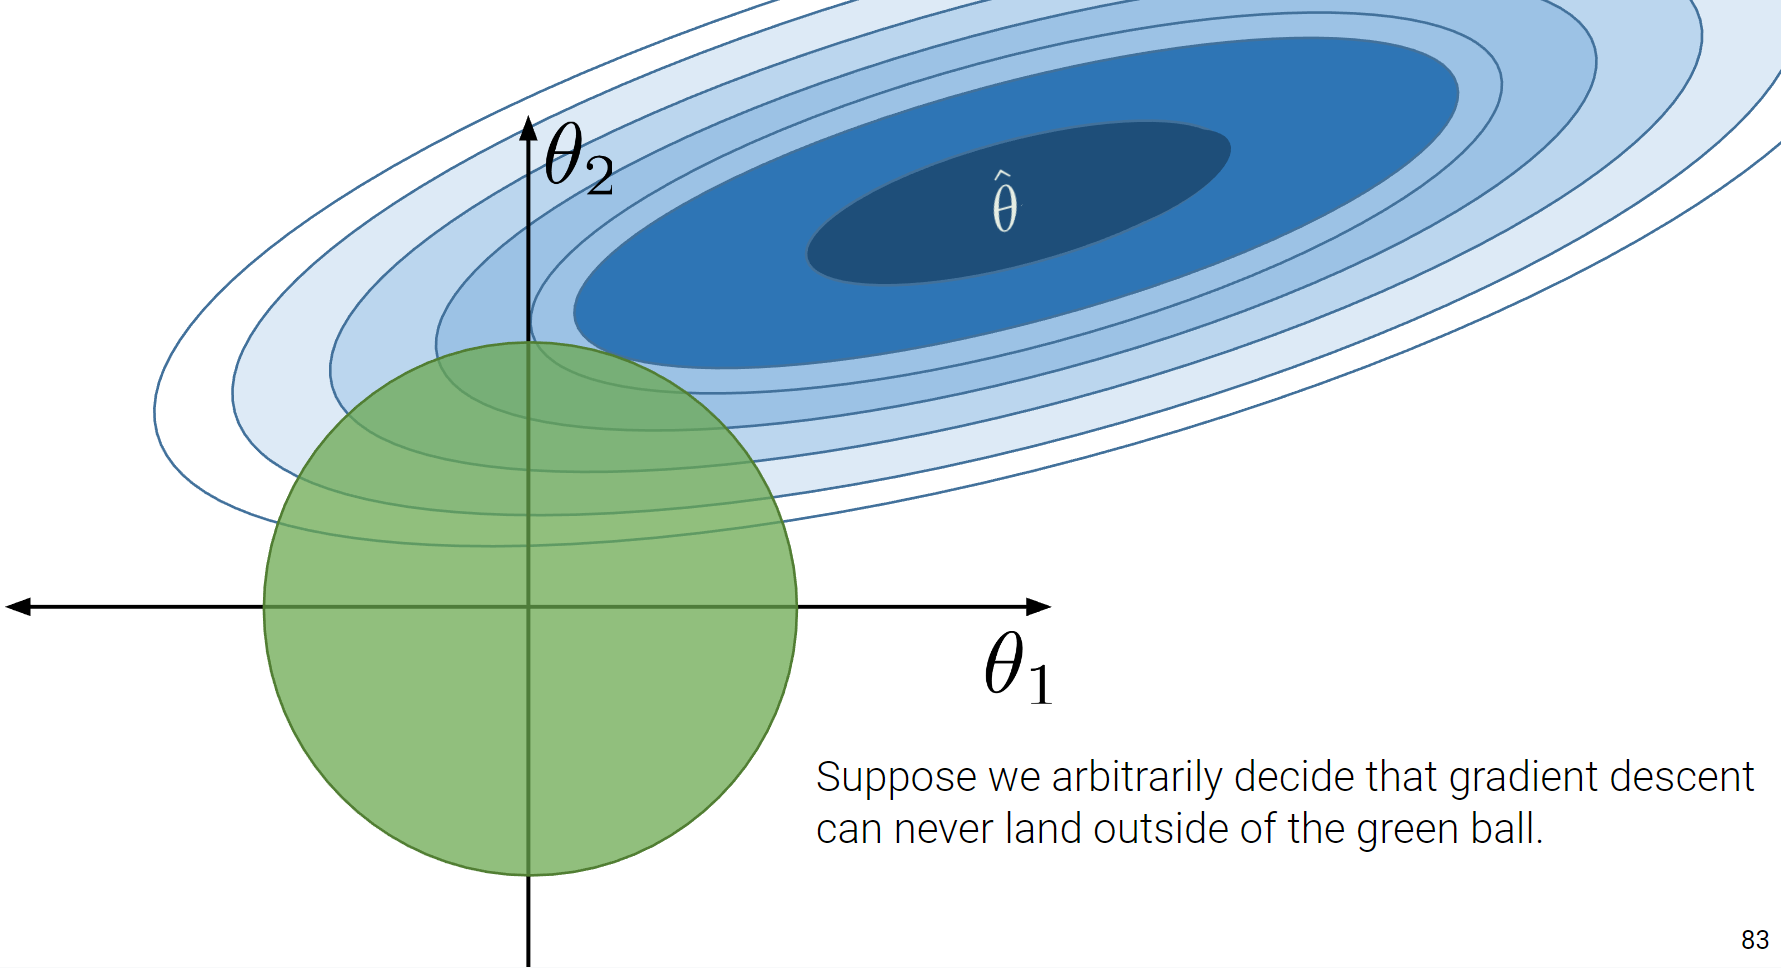
\includegraphics[scale=0.2]{figs/ln07/lin-reg-regularize.png}
    \end{center}
\end{ln-fig}

Now we may ask, how does the radius of this green circle tie in with reducing the complexity of a model. \\
When the green circle is small, we are limited into a less complex model, because the values of each parameters are more restrained. Under the extreme circumstance our green circle is essentially a point, the model would then output $0$ for any possible predictor variable, as the output prediction of model is bound within the green circle. \\
Here, we may also notice that $\theta_0$ is not involved in the model despite being involved in the multiple linear regression line. This would imply that reducing the green circle into a point produces a constant model that merely returns $\theta_0$ as its prediction, which as discussed before, is optimally the mean of every observed value. \\
On the other hand, the larger the green circle's radius is the closer our model behaves to the original model. This allows for more complexity than the previously mentioned constant model. \\
Noticeably then, overly small and overly large radius for the restraining circle each lead to unideal consequences.
\begin{bindenum}
    \item Small radius leads to a constant model with miniscule variance, where validation and training error are both high.
    \item Large radius leads to the original model of regression, which allows for large variance and in exchange brings high validation error with low training error.
\end{bindenum}

However, the nature of variables can lead to their parameters being naturally large. For example, variables that span between $1e-5$ and $1e-3$, perhaps due to unit or measurement, will naturally have larger parameters to help signify their significance in the regression model. \\
To prevent such issues, we should attempt to standardize each data by replacing every data entry with its z-score within its variable category:
\[z_k = \frac{x_k - \mu_k}{\sigma_k}\]
(This is also how the course COMPSCI 70 evaluate each students' performance on an exam, due to its average frequently being around 50\%).

\section{Choices of Regularization}
In other choices of regularization scheme, the circle can be substituted by other shapes.
The green shape on the visual at the beginning of prior section purposes to restrain the parameter size. Below, we will epxlore shapes other than circles that can also fulfill such duty. \\

\subsection{L2 Regularization (Ridge)}
Let us review the visualization of this scheme once again: 
\begin{ln-fig}[sidebyside]{L2 Regularization}{}
    \begin{center}
        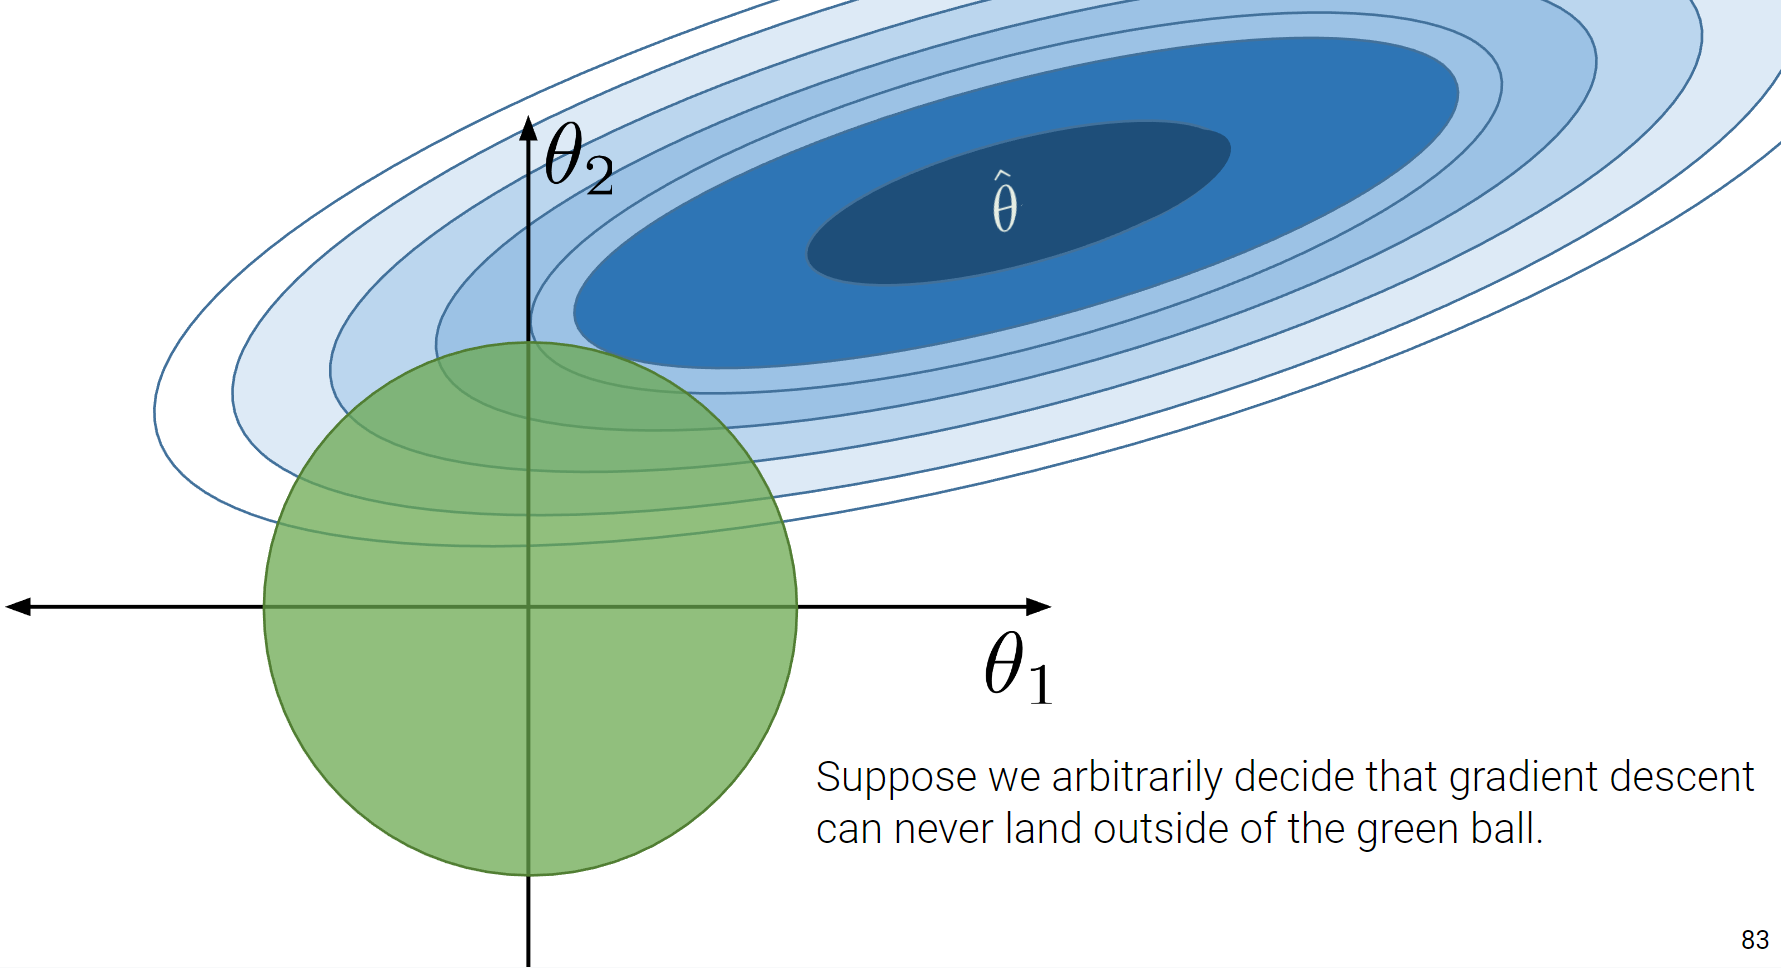
\includegraphics[scale=0.2]{figs/ln07/lin-reg-regularize.png}
    \end{center}
    \tcblower
    L2 Regularization is the scheme where we choose the green shape to be a circle around the origin. In this case, we attempt to minimize the empirical risk, paying attention to this constraint:
    \[\sum_i \theta_i^2 \leq r^2\]
    For an arbitrary, user-chosen $r$ as the radius of the green circle.
\end{ln-fig}

We can run ordinary least squares in the coursework's technology using a ``Ridge'' class as follows:
\setbox\codebox=\hbox{
    \begin{lstlisting}
    >>> from sklearn.linear_model import Ridge
    >>> ridge_model = Ridge(alpha = 10000)
    >>> #alpha is proportional to inverse of radius of
        regularization circle
    >>> ridge_model.fit(design_matrix, y)
    >>> ridge_model.coef_
    an array of optimal model parameters
    \end{lstlisting}
}
\begin{ln-code}{L2 Ridge Regularization in Python}{}
    \usebox\codebox
\end{ln-code}

The reason for which this class is named ``Ridge'' is because the OLS model with an L2 Regularization term is also called \textbf{Ridge Regression} in machine learning:
\begin{ln-define}{Ridge Regression Model}{}
    In a ridge regression model, we find parameters that minimize the following empirical risk as optimal:
    \[R(\theta) = \frac{1}{n}\sum_{i = 1}^n {{(y_i - (\theta_0 + \sum_{j = 1}^d \theta_j \Phi_{i, j}))}^2} + \alpha \sum_{k = 1}^d \theta_k^2\]
    The optimal solution is, for linear algebra that we will not discuss until EECS 127:
    \[\hat{\theta}_{ridge} = {(\X^T \X + n \alpha I)}^{-1} \X^T \Y\]
\end{ln-define}

\subsection{L1 Regularization (LASSO)}
In this scheme, we replace the circle with a cube:
\begin{ln-fig}[sidebyside]{L1 Regularization}{}
    \begin{center}
        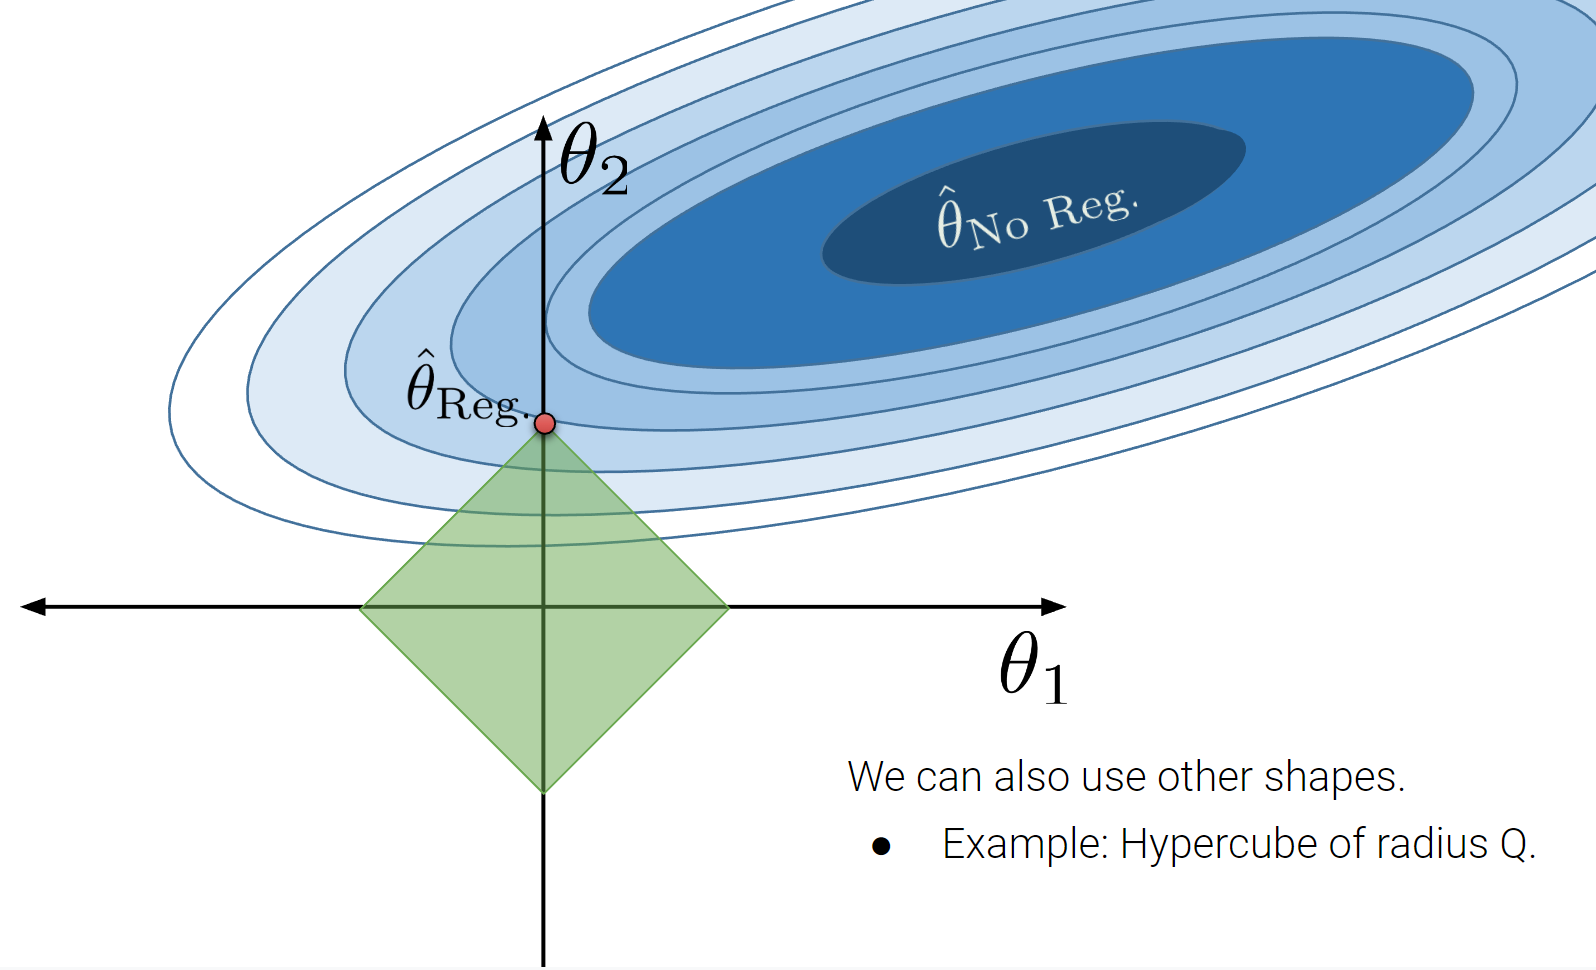
\includegraphics[scale=0.2]{figs/ln07/l1-regularize.png}
    \end{center}
    \tcblower
    Our empirical risk thus becomes:
    \[R(\theta) = \frac{1}{n}\sum_{i = 1}^n {{(y_i - (\theta_0 + \sum_{j = 1}^d \theta_j \Phi_{i, j}))}^2} + \alpha \sum_{k = 1}^d |\theta_k|\]
\end{ln-fig}
In the coursework technology, we may perform L1 regularization on OLS, otherwise known as LASSO Regularization, as noted below:
\setbox\codebox=\hbox{
    \begin{lstlisting}
    >>> from sklearn.linear_model import Lasso
    >>> lasso_model = Lasso(alpha = 10)
    >>> lasso_model.fit(design_matrix, y)
    >>> lasso_model.coef_
    an array of optimal model parameters
    \end{lstlisting}
}
\begin{ln-code}{L1 LASSO Regularization in Python}{}
    \usebox\codebox
\end{ln-code}
\textbf{LASSO Regularization}, or ``Least Absolute Shrinkage and Selection Operator'', tend to involve many zeros in its optimal parameters. In other words, it only chooses a subset of features to use in its regression model. \\

\subsection{Summary of Regularization Choices}
\begin{center}
    \begin{tabular}{c|ccc|c|c}
        Name & Model & Loss & Reg. & Empirical Risk & Solution \\
        \hline
        OLS & $\hat{\Y} = \X \theta$ & L2 & None & $\frac{1}{n}{||\Y - \X \theta||}_2^2$ & $\hat{\theta}_{OLS} = {(\X^T \X)}^{-1} \X^T \Y$ \\
        Ridge & $\hat{\Y} = \X \theta$ & L2 & L2 & $\frac{1}{n}{||\Y - \X \theta||}_2^2 + \lambda \sum_{j = 1}^d \theta_j^2$ & $\hat{\theta}_{OLS} = {(\X^T \X + n\lambda I)}^{-1} \X^T \Y$ \\
        LASSO & $\hat{\Y} = \X \theta$ & L2 & L1 & $\frac{1}{n}{||\Y - \X \theta||}_2^2 + \lambda \sum_{j = 1}^d |\theta_j|$ & no closed form
    \end{tabular}
\end{center}

\newpage
\part{Probability Theories in Modeling}
\chapter{DATA C100: A Survey on Random Variables}

\section{Defining Random Variables and Distributions}
In data science and statistics, we frequently discuss random experiments and random results: they are indeed some variable, but with a randomness in their values. We then specify these variables under the terminology:
\begin{ln-define}{Random Variable}{}
    A \textbf{random variable} is a numerical function for some random result. Its value on any given draw is called a realization.
    Each random variable is defined with a domain and a range:
    \begin{bindenum}
        \item The \textbf{domain} of a random variable is all possible random samples from our random processes.
        \item The \textbf{range} of a random variable depends on what the variable measures, but can be either discrete or continuous.
    \end{bindenum}
\end{ln-define}
For example, let $X$ be a random variable denoting the sum of two fair dice rolls. Then, this $X$ is discrete, and each value of $X$ would have some different probability. \\
Furthermore, the domain of this random variable would be all possible two-dice roll combinations, while the range would be the set $\{2, \dots, 12\}$.

These random variables can often be described under some larger framework. Many random variables come with or measure very similar properties, say ``the number of success in a binary experiment'' or ``the time it takes to perform some task for the first time''. \\
It would be convenient to provide frameworks for these general descriptions. This is what we refer to as \textbf{distribution}:
\begin{ln-define}{Distribution}{}
    The distribution of a random variable $X$ is a description of how its total probability is split over the range of $X$. \\
    In this case, the distribution defines a random variable, by designating for all $x \in range(X)$ on the value $\P[X = x]$.
\end{ln-define}
While many distributions will eventually be introduced in the COMPSCI 70 component for these notes, it would serve utility as well to introduce a list of distributions as follows:
\begin{bindenum}
    \item {
        Bernoulli(p), the Bernoulli distribution, also known as an indicator random variable:
        \[
            \begin{cases}
                \P[X = 1] = p \\
                \P[X = 0] = (1 - p)
            \end{cases}
        \]
    }
    \item {
        Binomial(n, p), the Binomial distribution, measures the number of Bernoulli trials with value $1$ out of $n$ trials performed.
    }
    \item {
        Uniform distribution, where probability of each value of range is equal; for example, the probability of rolling each possible value on a fair six-faced dice.
    }
    \item {
        Normal distribution, a Gaussian distribution used widely for its convenience and properties. Will introduce and discuss in depth at COMPSCI 70.
    }
\end{bindenum}

\section{Describing Random Variables: Expectation and Variance}
To define a random variable, we can use histograms and distributions. To summarize and describe a random variable, we discuss the expectation and variance of a random variable, both metrics we will define and discuss in this section.

Each distribution of the random variable has some center of mass, which otherwise is famously called the \textit{mean}. The formal terminology for the centroid of distribution is \textbf{expectation}. \\
\begin{ln-define}{Expectation}{}
    The expectation of a random variable $X$ is the weighted average of values of $X$, using the probabilities of values as weights. \\
    By definition, it is computed as:
    \[\E[X] = \sum_{x \in range(X)} x \P[X = x]\]
\end{ln-define}
Eventually, we will learn that expectation is the long run average of some random variable.

Meanwhile, we can also summarize the variability and the spread of a random variable via this metric called \textbf{variance},
\begin{ln-define}{Variance}{}
    The variance of a random variable $X$ is the expected squared deviation from the expectation of $X$. \\
    While this invokes the prior knowledge:
    \[\sigma = SD(X) = \sqrt{Var(X)}\]
    It presents that the variance of a random variable would be computationally defined as:
    \[Var(X) = \E[{(X - \E[X])}^2]\]
    which can also be simplified into:
    \[Var(X) = \E[X^2] - {\E[X]}^2\]
    via some derivation we show in COMPSCI 70 instead.
\end{ln-define}
The main usage of variance, as well as standard deviation due to their relevance, would be quantifying chance error in situations that require this measurement. For example, in a hypothesis test.

\section{Multiple Random Variables}
There are functions that use multiple random variables at once; however, these random variables' values can have underlying connections. To characterize these situations that make computation inconvenient, let us consider the following relationship between random variables. \\
Suppose we have random variables $X$ and $Y$, then their relationship may be described by one of the following:
\begin{bindenum}
    \item [1.] \textbf{Equal}: $X$ and $Y$ are equal if $X(s) = Y(s)$ for every sample $s$. This is otherwise expressed as $X = Y$.
    \item [2.] \textbf{Identically Distributed}: $X$ and $Y$ are identifically distributed if they have the same distribution. Identical distribution is implied by equivalence.
    \item [3.] \textbf{IID}: $X$ and $Y$ are independent and identially distributed if $X$ and $Y$ are identially distributed and are independent of each other.
\end{bindenum}
There may also be dependent random variables, where the value of $X$ influence the distribution of $Y$ as some conditional probability. However, that is not in the concern of DATA C100.

Now that we have clarified relationships involving multiple random variables, let us explore how the expectations and variances of related random variables behave:
\begin{ln-define}{Properties of Expectation}{}
    There are the following useful properties for expectation:
    \begin{bindenum}
        \item $\E[aX + b] = a\E[X] + b$
        \item $\E[X + Y] = \E[X] + \E[Y]$
        \item For a non-linear $g$, in general, $\E[g(X)] \neq g(\E[X])$.
    \end{bindenum}
\end{ln-define}
And following that,
\begin{ln-define}{Properties of Variance}{}
    There are the following useful properties for variance:
    \begin{bindenum}
        \item $Var(aX + b) = a^2 Var(X)$
        \item $Var(X_1 + X_2) = Var(X_1) + Var(X_2) + 2Cov(X, Y)$
    \end{bindenum}
    \begin{ln-define}{Covariance}{}
        The covariance of random variables $X$ and $Y$ measures the linear correlation between $X$ and $Y$, mathematically denoted as:
        \[Cov(X, Y) = \E[(X - \E[X])(Y - \E[Y])]\]
        where uncorrelated $X$ and $Y$ have zero correlation and covariance. \\
        It is important to note that independent random variables are uncorrelated of each other, but uncorrelated random variables can remain dependent. \\
        An interesting case for the above description appears in COMPSCI 70.
    \end{ln-define}
\end{ln-define}

\section{Bernoulli and Binomial Random Variables}
By prior statements, we may notice that the properties of binomial random variables is tightly connected to the properties of Bernoulli random variables. \\
In that case, it is more logical to introduce Beroulli random variables first:

\subsection{Bernoulli Random Variables}
Let us review the definition of Bernoulli random variables:
\begin{ln-define}{Bernoulli Random Variable}{}
    A random variable $X$ whose distribution follows some Bernoulli distribution $Bernoulli(p)$ is a Bernoulli random variable. \\
    In a Bernoulli distribution characterized by parameter $p$: $Bernoulli(p)$,
    \[
        \begin{cases}
            \P[X = 1] = p \\
            \P[X = 0] = 1 - p
        \end{cases}
    \]
\end{ln-define}
We may then calculate its expectation to be:
\[\E[X] = 1 \cdot p + 0 \cdot (1 - p) = p\]
And its variance to then be:
\begin{align*}
    Var(X) &= \E[X^2] - {\E[X]}^2 \\
    &= (1^2 \cdot p + 0^2 \cdot (1 - p)) - {(1 \cdot p + 0 \cdot (1 - p))}^2 \\
    &= p - p^2 = p(1 - p)
\end{align*}

\subsection{Binomial Random Variables}
Having performed some analysis on the Bernoulli distribution, let's now introduce Binomial distribution:
\begin{ln-define}{Binomial Random Variables}
    A random variable $X$ is binomial if its distribution is some binomial distribution $Binomial(n, p)$. \\
    A binomial random variable measures the number of value-$1$ Bernoulli trials with success probability $p$ out of all $n$ such Bernoulli trials. \\
    The distribution is defined as:
    \[
        \P[X = k] = \binom{n}{k} p^k {(1 - p)}^{(n - k)}
    \]
\end{ln-define}
We may then calculate its expectation to be:
\[\E[X] = np\]
for the variable $X$ is essentially a sum of $n$ IID Bernoulli random variables $X_i$
And its variance in turn:
\begin{align*}
    Var(X) &= Var(X_1 + \cdots + X_n) \\
    &= Var(X_1) + \cdots + Var(X_n) \\
    &= np(1 - p)
\end{align*}

\newpage
\chapter{DATA C100: Estimators, Bias, and Variance}

We have now find many ways to compute and summarize random variable via statistical and mathematical means, as outlined in A Survey on Random Variables and to be performed in future chapters. \\
However, data science per se often concern with another issue: sampling. While we may obtain the distribution of some random sample we acquire, we do not necessarily then recognize the distribution of a population. \\
So the essential question this chapter's contents revolve around would then be:
\begin{center}
    ``Can we infer or estimate the properties of a population based on the distribution of our samples?''
\end{center}

\section{Sample Statistics}
Consider that each datapoints in our sample is some IID random variable drawn from the population distribution. \\
Then, we may consider the statistics of this sample to be a random variable as well, as the possible samples themselves are driven from random experiments and will serve as the domain of these random-variable styled statistics.

Here, an incredibly practical theorem would then answer the question we threw at the beginning of the chapter.
\begin{ln-theorem}{Central Limit Theorem}{}
    Regardless of the population that samples are drawn from, if an IID sample of size $n$ is large, the probability distribution of the sample mean is roughly normal with mean $\mu$, standard devaition $\frac{\sigma}{\sqrt{n}}$. \\
    Here, $\mu$ is the population mean, and $\sigma$ is population standard deviation.
\end{ln-theorem}
A much formal introduction to Central Limit Theorem will be performed in the last few chapters for COMPSCI 70.

We may then, along the help of Central Limit Theorem, define the ``average sample'' that a population possibly acquires:
\begin{ln-define}{Sample Mean}{}
    Consider an IID sample $X_1, \dots, X_n$ drawn from numerical population with mean $\mu$, standard deviation $\sigma$, then the sample mean is a sample defined mathematically as:
    \[
        \overline{X_n} = \frac{1}{n} \sum_{i = 1}^n X_i
    \]
    Where we may then compute the expectation and variances of this sample mean to be:
    \begin{align*}
        \E[\overline{X_n}] &= \frac{1}{n} \sum_{i = 1}^n \E[X_i] \\
        &= \frac{1}{n} (n \mu) = \mu
    \end{align*}
    Meanwhile,
    \begin{align*}
        Var(\overline{X_n}) &= \frac{1}{n^2} \sum_{i = 1}^n Var(X_i) \\
        &= \frac{1}{n^2} n \sigma^2 = \frac{\sigma^2}{n} \\
        SD(\overline{X_n}) &= \frac{\sigma}{\sqrt{n}}
    \end{align*}
\end{ln-define}
The performance of Central Limit Theorem in realistic constraints is very dependent on the ambiguity in its description, ``a large $n$''. \\
What is the demand on the size of $n$ for CLT to work properly by description and present us some convenient normal distribution? \\
This would, in fact, depend on the skewness of population. If the population is roughly symmetric and unimodal, for example, the required value of $n$ becomes remarkably small. Otherwise, a large $n$ would still be required.

The use of sample mean as a statistic is to serve as an estimation of population mean: we consider the collaborative mean and variance of multiple samples to be a good estimate for that of the population. \\
But before discussinf the sample mean as an estimation, we should first switch gears and explore the concept of ``estimation'' in the context of modeling: that is, the work of inference.

\section{Prediction and Inference in Modeling}
A model is constructed for two dominant reasons:
\begin{bindenum}
    \item \textbf{Prediction}: The model offers a prediction for the response of an unseen data entry.
    \item \textbf{Inference}: Extracting conclusions about the underlying relationship between predictor features and responses from a model's inner settings and parametric properties.
\end{bindenum}
Then, in the context of modeling, the work of estimation as addressed in prior section to infer about population parameters given some random sample. This is otherwise called ``statistical inference''.

\subsection{Estimator and Bias-Variance Tradeoff}
The performance of an estimator variable can be assessed at the following perspectives:
\begin{bindenum}
    \item \textbf{Bias}: Does the estimator variable offer the right answer (value of estimated parameter) on average?
    \item \textbf{Variance}: What is the variability of the estimator's answer?
    \item \textbf{Risk}: How close is the work of estimator to the parameter it estimates?
\end{bindenum}
All of which offer some mathematical quantification to evaluate the estimator's performance.
\begin{ln-define}{Bias of Estimator}{}
    The bias of an estimator measures its average deviation from the true value (parameter):
    \[
        Bias(\hat{\theta}) = \E[\hat{\theta} - \theta] = \E[\hat{\theta}] - \theta
    \]
    Because the sample mean's average is $\E[\hat{\theta}] = \mu$, directly equivalent to the population mean, the sample mean served as an unbiased estimator.
\end{ln-define}
\begin{ln-define}{Risk of Estimator}{}
    The risk of the estimator can be expressed via some loss function like MSE as:
    \[
        MSE(\hat{\theta}) = \E[{(\theta - \hat{\theta})}^2]
    \]
    And if the estimator $\hat{\theta}$ is unbiased, we may learn that $\E[\hat{\theta}] = \theta$, making the risk of an estimator its variance.
\end{ln-define}
In the case that the estimator is not unbiased, we can then decompose MSE risk of the estimator as follows:
\begin{align*}
    b &= \E[\hat{\theta}] - \theta \\
    MSE(\hat{\theta}) &= \E[{(\hat{\theta} - \theta)}^2] \\
    &= \E[{(\hat{\theta} - \E[\hat{\theta}] + b)}^2] \\
    &= \E[{(\hat{\theta} - \E[\hat{\theta}])}^2] + b^2 + 2b\E[(\hat{\theta} - \E[\hat{\theta}])] \\
    &= b^2 + Var(\hat{\theta})
\end{align*}
We call this result the \textbf{Bias-Variance Decomposition}.

\subsection{Estimation Error for Modeling}
Let us apply the notion of ``estimation'' onto choosing model relationships. \\
Say, that the response variable $Y$ is to predicted by some expression:
\[Y = g(x) + \epsilon\]
for some $g$ that estiamtes the true relationship between $x$ and $Y$. Then, $\epsilon$ would represent some random error or noise that are expectedly zero-mean and IID across individual datapoints.
From there, some model for predictions based on observed samples are created: $\hat{Y}(x)$, which once again estimates the true relationship that $g$ is. Evidently, at every set of predictor features $x$, our prediction for the response would then be $\hat{Y}(x)$. \\
Naturally, these estimative models will then also have their own set of optimal parameters to minimize some loss; this fact we will mathematically express here for:
\[\hat{Y}(x) = f_{\hat{\theta}}(x)\]

\section{Bias-Variance Tradeoff}
Let us combine the prior subsections' work to discuss the essential phenomenon and guideline of model training: bias-variance tradeoff, which outlines the tradeoff of model characteristics that determine the overfitting inclinations of models.

From prior work, we can discover the bias-variance decomposition of some \textbf{model risk} (the risk of a model). \\
Model risks are composed of:
\begin{bindenum}
    \item \textbf{Observation Variance}, noted by the random noise $\epsilon$ found from observation; once again, expectedly zero-mean.
    \item \textbf{Model Variance}, the variance that model presents with the random samples it can utilize.
    \item \textbf{Model Bias}, as our model will have some deviation with the true estimated relationship $g$.
\end{bindenum}
And by prior work we have understood that:
\[
    \text{model risk} = \text{observation variance} + {(\text{model bias})}^2 + \text{model variance}
\]
Let us then discuss these aspects of model risk:
\begin{ln-define}{Observation Variance}{}
    Observation Variance is the variance of random error, mathematically denoted as:
    \[\sigma^2\]
    which originates from measurement error and noise-behaving missing information. \\
    While observation variance can be reduced via more precise measurements, this is often beyond the control of scientists.
\end{ln-define}
\begin{ln-define}{Model Variance}{}
    Since our fitted model $\hat{Y}$ is on a random sample, the deviations of possible random samples to fit model on would present different models. \\
    This varaince of our prediction at a fixed $x$ is known as model variance, mathematically denoted as:
    \[Var(\hat{Y(x)})\]
    Model variance can originate from overfitting, where small differences in random samples lead to huge deviations in some fitted model due to the models being overfitted to their respective random training samples. \\
    To reduce model variance, one may reduce model complexity (as a method to inhibit overfitting), as well as preventing the model to fit the observation variance and noises.
\end{ln-define}
\begin{ln-define}{Model Bias}{}
    The model bias is the difference between our predicted response and the true value of response, mathematically defined as:
    \[\text{model bias} = \E[\hat{Y(x)}] - g(x)\]
    Here, bias is an average measure for some fixed $x$, just as model variance is presented. \\
    By the nature of bias being ``estimation minus real'', a positive bias expresses overestimation, while negative bias expresses underestimation. The opposite logic was applied on residuals. \\
    Overall, model bias can originate from underfitting, as well as from the lack of domain knowledge that a model requires to operate well. To reduce model bias, one can increase the model complexity and involve domain knowledge to construct better prioris for prediction work.
\end{ln-define}
Therefore, summarizing the above, we see that the bias-variance decomposition for some model risk can be summarized mathematically as:
\[
    \E[{(Y - \hat{Y}(x))}^2] = \sigma^2 + {(\E[\hat{Y}(x)] - g(x))}^2 + Var(\hat{Y}(x))
\]
as paralleling the prior statement:
\[
    \text{model risk} = \text{observation variance} + {(\text{model bias})}^2 + \text{model variance}
\]
Therefore, we obtain some important conclusions:
\begin{bindenum}
    \item As models increase in complexity, they overfit and present higher model variance.
    \item As models decrease in complexity, they underfit and present higher model bias.
    \item Observation variance is fundamentally irereducible.
    \item Model risk is a fixed constant due to it being some expectation of random variable.
\end{bindenum}
Consequentially: when tuning a model, \textbf{either its bias or its variance increase}.

This leads to the famous diagram and saying of \textbf{Bias-Variance Tradeoff}:
\begin{ln-fig}{Bias-Variance Tradeoff, DATA C100}{}
    \begin{center}
        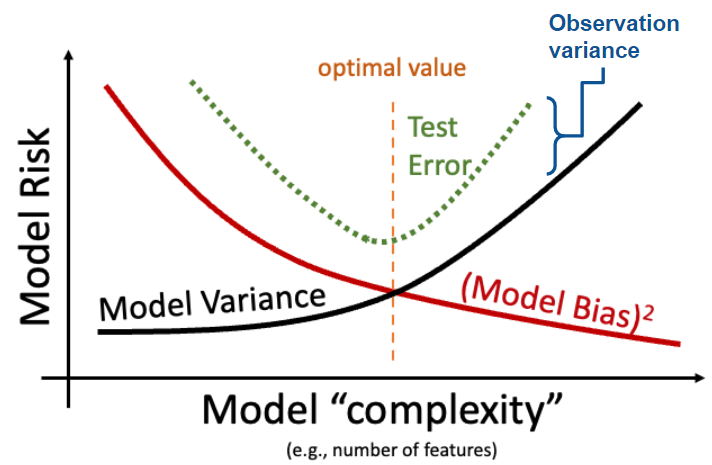
\includegraphics[scale=0.8]{figs/ln09/bv-tradeoff.png}
    \end{center}
\end{ln-fig}

\newpage
\chapter{DATA C100: Causal Inference and Confouding}

\section{Interpretation of Models}
As previously mentioned, models exist not only for prediction, but also inference. \\
The structure of a model would influence how easy interpretations and inferences can be produced. In this case, since linear regression is a rather conceptually simple model, we will explain the concept of inference using it.

For a linear regression method, we estimate the true relationship between a response and its predictors using a mathematically optimal set of parameters $\hat{\theta}$ specific to the model. \\
That model is:
\[
    f_{\hat{\theta}}(x) = \hat{\theta}_0 + \hat{\theta}_1 x_1 + \cdots + \hat{\theta}_p x_p
\]
Here, the parameters, which essentially have defined the model, is important for inference. \\
For example, if a predictor variable $x_i$ has some estimated parameter of it $\hat{\theta}_i$ that has a zero value, it means the value of $x_i$ does not contribtue to the response variable; therefore, does not affect the response value. \\
We may then test the insignificance of $x_i$ by performing hypothesis testing on the paramter $\theta_i$ as follows:
\begin{bindenum}
    \item \textbf{Null Hypothesis}: The true parameter $\theta_i$ is $0$.
    \item \textbf{Alternate Hypothesis}: The true parameter $\theta_i$ is not $0$.
\end{bindenum}
We will then perform some bootstrapping to produce several models, and see how the confidence interval of estimated parameters $\theta_i$ across each model present. \\
If the confidence interval for our p-value cutoff does indeed involve $0$, we would accept the null hypothesis; otherwise, we find enough reason to reject the null hypothesis.

Is there some mathematical problem that prevents interpretation of invidual predictor variables' significance? Yes. 
If some predicted variables are related to each other, then our interpretation, which attempts to detect the significance of an individual variable with the response, would fail its purpose. \\
We can no longer test one variable by holding others constant, but this is essential to causal inference: inferring whether a specific predictor variable was the cause of some alteration in a response variable. \\
This problem is called \textbf{collinearity}:
\begin{ln-define}{Collinearity}{}
    When a feature can be predicted accurately as a linear function of others, collinearity exists in the dataset. 
    This causes small changes in the data sample to lead to big changes in the estimated slopes of predictor variables. \\
    Collinearity is implied by the noninvertibility of design matrix as well.
\end{ln-define}

\section{Causal Inference}
Here is a short section for outlining the philosophical difference between ``correlation'' (association) and ``causation''.

Questions about correlation look for some mathematical relationship between one variable and another, but causal questions discuss the effects of some intervention. Regression coefficients cannot stand for effects. \\
In other words, correlation questions ask: ``Does the increase of some value coexist with the alteration of some other value, and how significantly?'' \\
But causation would ask: ``Does the increase of some value cause the significant observed alteration of some other values'', and involve counterfactual questions asking if the converse holds true or not to validify the causal effect.

At times, confounding variables appear. \\
A \textbf{confounder} is a variable that affects both the treatment and the response, which distorts the correlation between them. While the common assumption of data science studies would assume that all confounders are observed, confounders can still trigger substantial collinearity in the offered dataset.

Let us now move on to the practical aspects of causal inference. \\
In prediction, we have used the following terminologies:
\begin{bindenum}
    \item \textbf{Response} (Y): what is to be predicted.
    \item \textbf{Predictors} (X): what is to be inputted.
\end{bindenum}
But, in causal inference, we will modify these terminologies slightly along the context of inference problems:
\begin{bindenum}
    \item \textbf{Response} (Y): the outcome of interest.
    \item \textbf{Treatment} (T): the variable we might intervene on.
    \item \textbf{Covariate} (X): potential confounders.
\end{bindenum}
For the scope of this course, we will focus on $T$ as indicator variables. \\
Each datapoint of our model will then be involved as tuples of following format:
\[
    (x_i, T_i, Y_i (0), Y_i (1))
\]
where the variables respectively stand for covariates, treatment, treated outcome ($y_i$ if $T_i = 1$), and control outcome ($y_i$ if $T_i = 0$). \\
This model is known as the \textbf{Neyman-Rubin Causal Model}. However, since we only ever observe one of the potential outcome (treated or control). There are limitations upon which we estimate the true effects of a treatment. \\
For example, on the metric \textbf{Average Treatment Effect}:
\[ATE = \E[Y(1)] - \E[Y(0)]\]
we cannot just take a sample mean as an estimator, because we only ever observe one potential outcome per datapoint.

Now, how do we assign treatments to different groups to avoid statistical bias? \\
While randomized experiments are theoretically suitable approaches, they are often unethical or impractical in realistic contexts. Therefore, scientists have long preferred its alternative: \textbf{observational studies}. \\
In observational studies, we merely observe the effects of treatments without much priori or beforehand knowledge on possible inherent deviations between ``treatment group'' and ``control group''. This develops into unmeasured confounders, which also do not appear ideal for accurate inferences. \\
But, in other words, we now just have to find a way to mitigate confounders.

\section{Covariate Adjustment}
The aforementioned great assumption for confounders has been \textbf{ignorability assumption}; once again, it states that all important confounders are in the data set. \\
However, such approach is very fragile: it breaks if important covariates are missing, or if the true dependence on $x$ is nonlinear. \\
Albeit we may also come up with some model that ought to include them, additional ssumptions would be needed for the model to finally work.

There still exist other methods for alleviating confounders, where many of these methods would model treatment as a function of covariates, if not modeling the outcome as a function of both covariate and treatment. \\
One notable example, meanwhile, would be regression discontinuity. Such a method has a running variable $x$, and let $T = 1$ if and only iff $x > \text{threshold}$. This would allow us to have two separate regression models piecewise-concatenated together. \\
This method would avoid the confounding issues as treatment becomes a determinstic function of covariates, estimand becomes ATE for units near the threshold, and is widely used across real-life problems such as clinical threshold for treatment and PSAT/NMSQT cutoffs.
\begin{ln-fig}{Regression Discontinuity, DATA C100}{}
    \begin{center}
        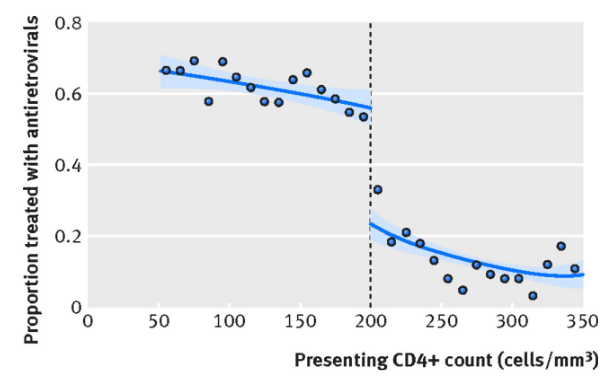
\includegraphics[scale=0.8]{figs/ln10/reg-discont.png}
    \end{center}
\end{ln-fig}

%\end{comment}
\end{document}
